% 
%% Copyright 2007, 2008, 2009 Elsevier Ltd
%% 
%% This file is part of the 'Elsarticle Bundle'.
%% ---------------------------------------------
%% 
%% It may be distributed under the conditions of the LaTeX Project Public
%% License, either version 1.2 of this license or (at your option) any
%% later version.  The latest version of this license is in
%%    http://www.latex-project.org/lppl.txt
%% and version 1.2 or later is part of all distributions of LaTeX
%% version 1999/12/01 or later.
%% 
%% The list of all files belonging to the 'Elsarticle Bundle' is
%% given in the file `manifest.txt'.
%% 

%% Template article for Elsevier's document class `elsarticle'
%% with numbered style bibliographic references
%% SP 2008/03/01

\documentclass[preprint,12pt]{elsarticle}

%% Use the option review to obtain double line spacing
%% \documentclass[authoryear,preprint,review,12pt]{elsarticle}

%% Use the options 1p,twocolumn; 3p; 3p,twocolumn; 5p; or 5p,twocolumn
%% for a journal layout:
%% \documentclass[final,1p,times]{elsarticle}
%% \documentclass[final,1p,times,twocolumn]{elsarticle}
%% \documentclass[final,3p,times]{elsarticle}
%% \documentclass[final,3p,times,twocolumn]{elsarticle}
%% \documentclass[final,5p,times]{elsarticle}
%% \documentclass[final,5p,times,twocolumn]{elsarticle}

%% For including figures, graphicx.sty has been loaded in
%% elsarticle.cls. If you prefer to use the old commands
%% please give \usepackage{epsfig}

%% The amssymb package provides various useful mathematical symbols
\usepackage{xspace}
\usepackage{amssymb}
\usepackage{amsmath}
\usepackage{subcaption}
\usepackage[printonlyused]{acronym}
%%
\acrodef{AHB}[AHB-PNW]{Advanced Hardwood Biofuels Northwest}
\acrodef{BCAM}{Bioenergy Crop Adoption Model} 
\acrodef{CCSM3}{Community Climate System Model version 3}
\acrodef{CDL}{Cropland Data Layer}
\acrodef{GBSM}{Geospatial Bioenergy Systems Model}
\acrodef{GIS}{Geographical Information System}
\acrodef{IPCC}{Intergovernmental Panel on Climate Change}
\acrodef{mmu}{minimum mapping unit}
\acrodef{NASS}{National Agricultural Statistics Service}
\acrodef{NLCD}{National Land Cover Dataset}
\acrodef{NRCS}{Natural Resources Conservation Service, Department of Agriculture}
\acrodef{NREL}{National Renewable Energy Laboratory}
\acrodef{PNW}{Pacific Northwest}
\acrodef{PRISM}{Parameter-elevation Relationships on Independent Slopes Model} 
\acrodef{SRWC}{short rotation woody crops}
\acrodef{STATSGO}{State Soil Geographic}
\acrodef{USGS}{United States Geological Survey}
\acrodef{SECRETS}{Stand to Ecosystem CaRbon and EvapoTranspiration
Simulator}
%% 3PG acronyms
\acrodef{3pg}[\textsc{3PG}]{Physiological Principles in Predicting Growth}
\acrodef{BLcond}[\ensuremath{BL_{cond}}]{Boundary layer conductance}
\acrodef{dbh}[\ensuremath{dbh}]{Diameter at Breast Height}
\acrodef{DOB}[\ensuremath{DOB}]{Basal Diameter}
\acrodef{LAIt}[\ensuremath{LAI_{T}}]{Target Leaf Area Index}
\acrodef{LAI}[\ensuremath{LAI}]{Leaf Area Index}
\acrodef{NPPdef}[\ensuremath{NPP_{def}}]{$NPP$ deficit}
\acrodef{NPPt}[\ensuremath{NPP_{T}}]{Target Productivity}
\acrodef{NPP}[\ensuremath{NPP}]{Net Primary Productivity}
\acrodef{RP}[\ensuremath{RP}]{Root Productivity}
\acrodef{Rdp}[\ensuremath{R_{\Delta}}]{monthly root contribution}
\acrodef{Re}[\ensuremath{e_{R}}]{root conversion efficiency}
\acrodef{SLA}[\ensuremath{SLA}]{Specific Leaf Area}
\acrodef{WF}[\ensuremath{W_F}]{Foliage biomass}
\acrodef{WS}[\ensuremath{W_S}]{Stem biomass}
\acrodef{WR}[\ensuremath{W_R}]{Root biomass}
\acrodef{W}[\ensuremath{W}]{Plant biomass}
\acrodef{dRres}[\ensuremath{\Delta R_{res}}]{Residual root contribution}
\acrodef{dW}[\ensuremath{\Delta W}]{Total Monthly Growth}
\acrodef{fSW}[\ensuremath{f_\Theta}]{soil water limiter}
\acrodef{fAge}[\ensuremath{f_{age}}]{age growth limiter}
\acrodef{fNutr}[\ensuremath{f_{nutr}}]{nutritional limiter}
\acrodef{fT}[\ensuremath{f_T}]{temperature limiter}
\acrodef{fi}[\ensuremath{f_i}]{Generic growth limiters}
\acrodef{k}[\ensuremath{k}]{radiation extinction coefficient}
\acrodef{lf}[\ensuremath{lf}]{Litter fall}
\acrodef{pRx}[\ensuremath{x_{pR}}]{maximum root fraction}
\acrodef{pR}[\ensuremath{p_R}]{Root allocation}
\acrodef{pfs}[\ensuremath{p_{FS}}]{foliage to stem allocation fraction}
\acrodef{VI}[\ensuremath{VI}]{Volume Index}
\acrodef{sps}[\ensuremath{n_{stems}}]{Stems per stump}
\acrodef{cancover}[\ensuremath{CanCover}]{canopy coverage}
\acrodef{LA}[\ensuremath{LA}]{Leaf Area per stem}
\acrodef{swc}[\ensuremath{\Theta_{c}}]{$f_\Theta$ constant}
\acrodef{swp}[\ensuremath{\Theta_{P}}]{$f_\Theta$ power}
\acrodef{maxAWS}[\ensuremath{S_x}]{Maximum available soil water}
\acrodef{AWS}[\ensuremath{S}]{Available soil water}

% Tests
%\acrodef{HW1}{}
%\acrodef{HW2}{Hardwood Default in Coppice}


\usepackage{unitsdef}
%\newcommand{\degree}{\ensuremath{{}^{\circ}}\xspace}

%% The amsthm package provides extended theorem environments
%% \usepackage{amsthm}

%% The lineno packages adds line numbers. Start line numbering with
%% \begin{linenumbers}, end it with \end{linenumbers}. Or switch it on
%% for the whole article with \linenumbers.
\usepackage{tabularx}
\usepackage{lineno}
\usepackage{graphicx}
\usepackage{color}
\usepackage{hyperref}
\pdfpagebox5
\usepackage{pgfplots}
\usepgfplotslibrary{dateplot}



\journal{Biomass \& Bioenergy}

\begin{document}

\begin{frontmatter}

%% Title, authors and addresses

%% use the tnoteref command within \title for footnotes;
%% use the tnotetext command for theassociated footnote;
%% use the fnref command within \author or \address for footnotes;
%% use the fntext command for theassociated footnote;
%% use the corref command within \author for corresponding author footnotes;
%% use the cortext command for theassociated footnote;
%% use the ead command for the email address,
%% and the form \ead[url] for the home page:
%% \title{Title\tnoteref{label1}}
%% \tnotetext[label1]{}
%% \author{Name\corref{cor1}\fnref{label2}}
%% \ead{email address}
%% \ead[url]{home page}
%% \fntext[label2]{}
%% \cortext[cor1]{}
%% \address{Address\fnref{label3}}
%% \fntext[label3]{}

\title{Modeling Poplar Growth as a Short Rotation Woody Crop for Biofuels in the Pacific Northwest}

%% use optional labels to link authors explicitly to addresses:
%% \author[label1,label2]{}
%% \address[label1]{}
%% \address[label2]{}

\author[lawr]{Q. J. Hart}
\author[cf]{P.W. Tittmann}
%\author[plant]{B.L. Yeo}
%\author[lawr]{J. R. Merz}
%\author[pfc]{A. Cooke}
\author[bioag]{V. Bandaru}
\author[bioag]{B. M. Jenkins}

\address[lawr]{Dept. of Land, Air, and Water, University of California, Davis, USA\fnref{lawr}}
%\address{Precision Forestry Cooperative, University of Washington, USA\fnref{pfc}}
%\address{Department of Plant Sciences, University of California, Davis, USA\fnref{plant}}
\address[cf]{Center for Forestry, University of California, Berkeley, USA\fnref{cf}}
\address[bioag]{Dept. of Biological and Agricultural Engineering, University of California, Davis, USA\fnref{bioag}}

\begin{abstract}
  Predicting the economic viability and environmental sustainability
  of a biofuels industry based on intensively cultivated \acf{SRWC}
  requires spatial predictions of growth and yield under various
  environmental conditions and across large regions.  The \ac{3pg}
  model was modified to evaluate the growth and yield of coppiced
  poplar (\emph{Polulus spp}).  This included an additional biomass
  partitioning method and developing a sub-model which takes into
  account the impact of coppicing on post harvest regeneration,
  extending the applicability of the \ac{3pg} model to coppice
  management regimes.

  The parameterized model was applied to the entire Pacific Northwest
  of the United States, using appropriate climate and soil
  input data.  Results predict the yield of poplar cultivation at a
  spatial resolution of $\approx$ 64 km\textsuperscript{2} throughout
  the $\approx$8 million km\textsuperscript{2} of the study
  region. Existing agricultural cultivation patterns were used to
  estimate regional water availability for irrigation, and for
  non-irrigated regions, land cover features including ownership,
  slope , soil salinity and water table depth where used to select
  areas with a real potential to support a \ac{SRWC} plantation.

  Results can be integrated with other models that allow for
  optimizing crop selection and biorefinery site selection.  Important
  results include; an updated \ac{3pg} model for coppiced \ac{SRWC}
  plantings, estimates of biomass feedstock yields under different
  irrigation patterns and weather conditions, and estimates for
  feedstock availability when combined with crop adoption scenarios.

\end{abstract}

\begin{keyword}
%% keywords here, in the form: keyword \sep keyword
  Short rotation woody crops \sep Poplar \sep \ac{3pg} \sep Yield
  estimations \sep Pacific Northwest, USA.

%% PACS codes here, in the form: \PACS code \sep code

%% MSC codes here, in the form: \MSC code \sep code
%% or \MSC[2008] code \sep code 

\end{keyword}

\end{frontmatter}

%% \linenumbers

%% main text
\section{Introduction}
\label{sec:introduction}
%% Text of abstract
The \acf{AHB} is a consortium of university and industry partners
investigating the development of a sustainable hardwood biofuels
industry in Washington, Oregon, northern California, Idaho, and
western Montana in the United States.  Inspired in part by the
U.S. Energy Independence and Security Act 2022 targets for renewable
fuel, \ac{AHB} is carrying out research and development to support a
system for growing and converting hardwoods, such as hybrid poplars,
into liquid biofuels.  This research and development initiative has
focused on fuels fully compatible with existing liquid transportation
fuel infrastructure.

To support economic and environmental models for a biofuels industry,
spatial predictions of yield for \acf{SRWC} under various
environmental conditions are required throughout the entire \acf{PNW}
region.  The
\acf{3pg}~\cite{landsberg2010physiological,Landsberg1997,Sands2004}
model was utilized for this purpose.  Empirically based growth and
yield models for hybrid poplar have been used with some success in the
region~\cite{Clendenen1996}, however the samples used to develop
allometric relationships did not include coppice management.
\ac{SECRETS}~\cite{Sampson2001} is another process based model,
differing from \ac{3pg} in a number of ways, including biomass
production and aboveground partitioning~\cite{SurendranNair2012}.

The \ac{3pg} model was modified for \ac{SRWC}, particularly
for poplar plantation methodologies. The motivation for the use of
spatially resolved yield estimates is two-fold:
\begin{description}
\item[Biofuels production system optimization] Substantial investment
  is required to construct facilities capable of producing drop-in
  fuels~\cite{Parker2010a}. Capitalization of these facilities will
  depend upon a demonstrated
  consistent supply of feedstock. While spot or commodity markets may
  emerge to supply the demand for these facilities via bulk rail or
  marine supply chains, first mover facilities will
  likely depend on contracts with regional producers to supply a
  substantial percent of the facility demand. This analysis helps
  identify locations likely to have access to substantial local
  supply.
\item[Land use] The potential for displacement of food crops from
  agricultural lands is a possible outcome of expanding biofuel
  markets.
%PETER ! 
%\textbf{Citation}.
  The impacts associated with an increase in food prices on global
  food security raises ethical issues that relatively developed and
  food-secure societies must consider~\cite{Pimentel2008}. This
  exercise helps identify land not currently in food production that
  is potentially viable for \ac{SRWC} production.
\item
\end{description}

\ac{3pg} predicts total carbon based on photosynthetically active
radiation and is parameterized by variables relating to the tree, soil
(water availability) and weather data. It produces monthly estimates
of foliage stem and root biomass. In this analysis \ac{3pg} is run for
each pixel within a grid of the \ac{PNW}. Each pixel is modeled as a
stand with input parameters that vary with geography (soil,weather)
are used to parameterize the model. Modifications to the original
\ac{3pg} model include changes to the biomass partitioning, and the
inclusion of a root contribution to regrowth after coppicing.

A physiological growth model such as \ac{3pg} is advantageous because
it allows variation of growth parameters and assumptions regarding
management practices for poplar species.  In addition to biomass
growth and yield estimations, allocations for both above and below
ground biomass can be tracked for more complete life-cycle analysis of
the carbon budget related to the fuels.

The \ac{3pg} model has been used previously to model \ac{SRWC}
production. One~\cite{Amichev2010} used the \ac{3pg} to predict growth
of the Walker poplar hybrid (\textit{Populus deltoides} x
\textit{Populus nigra}) in Saskatchewan, Canada. This analysis did not
investigate the growth dynamics related to coppicing. In a separate
study~\cite{Deckmyn2004} the \ac{SECRETS} model was modified and
evaluated for coppice poplar production from two varieties under a
range of soil fertility conditions.  The \ac{SECRETS} coppice modified
paritioning fractions with the presence of a large root mass, one of
the outcomes of the coppicing model described here for \ac{3pg}.

The \ac{3pg} model~\cite{Headlee2012} has been deployed across several
states in the northern midwest United States to predict growth and
yield of hybrid poplar but did not evaluate the impact of coppice
management.  To date, the use of physiological growth models such as
the \ac{3pg} to evaluate spatial variability in yields of coppiced
\ac{SRWC} at the scale and extent of the results presented here has
not been attempted.

The original \ac{3pg} model does not include coppicing as a management
practice, which is problematic as it cannot reasonably account for
post-coppicing regrowth.  Coppicing of \ac{SRWC} has been widely
demonstrated to increase growth rates post-coppice in comparison to
un-coppiced stands~\cite{Verwijst1996,Afas2008a,Sennerby-Forsse1992}.
The extensions presented in this paper include coppicing with a
general sub-model that allows a monthly growth contribution from an
existing root mass.  The model specifies a relatively small
contribution of aboveground growth from the accumulated root mass
after coppicing in order to initiate the next cycle of
production~\cite{Deckmyn2004}.

With appropriate input information, the \ac{3pg} model can predict
yields for the entire Pacific Northwest study region, under various
irrigation scenarios.  When linked with models of crop adoption,
biofuel feedstock estimates are possible.

\section{Methods and Calculation}

The main goal of this study was to create spatially explicit poplar
growth potential for the \ac{PNW} that can reliably predict yield
from \ac{SRWC} plantations in the region.

The study area, the Pacific Northwest of the United States, includes
Washington, Oregon, northern California, Idaho, and western Montana.
A regular grid partitions the region.  The individual pixel size is
relatively coarse $8192$(m)$ \times 8192$(m). The spatial aggregation
will necessarily result in yield estimates that do not capture local
variability. However, the intent of the study is to identify areas of
high productivity within the study region. A coarse geographic unit
was selected to strike a balance between geographic specificity and
complexity of subsequent modeling steps not covered in this
paper. Another similar study~\cite{Headlee2012} used 32
km\textsuperscript{2} spatial resolution.

An Albers equal area projection with reference longitude 120\degree~W,
latitude 44\degree~N and parallels at 41\degree~N and 47\degree~N was
utilized.
%\footnote{\href{http://spatialreference.org/ref/sr-org/7260/}{http://spatialreference.org/ref/sr-org/7260/}}
Other input datasets (eg. climate, soils) were scaled to match the base
pixel size and raster projection. For example, the \ac{NLCD} dataset
used in this study, was originally imported and projected at a much
finer scale, $32 \times 32$ (m), then aggregated upwards and used to determine
proportion of landcover types within each 64 km\textsuperscript{2} unit~(Figure~\ref{fig:land}).

Data processing was carried out within a postgresql database, with the
postgis geospatial extensions~\cite{pgsql,Holl2009,postgis}.  The
\ac{3pg} model was implemented directly in the postgresql database via
user-defined functions adapted from the spreadsheet model procured
from the University of British Columbia \ac{3pg} support website
\footnote{\href{http://3pg.forestry.ubc.ca/}{http://3pg.forestry.ubc.ca/}}.The functions were implemented in JavaScript\texttrademark, so that a single library
could support this database (PostgreSQL), and an online application
documented in~\cite{Prilepova2014}.

\subsection{\acs{3pg} Model Formulation}
\label{sec:3pg}

The \ac{3pg} model takes as inputs weather data, soil parameters, site
factors, initial stocking conditions, management practices, and
species
definitions~\cite{landsberg2010physiological,Landsberg1997,Sands2004}.
\ac{3pg} runs at a monthly timestep. At each step the physiological
parameters are calculated and carried forward to the next month.
% Not sure bout this
% Addressing temporal resolution is requested by a reviewer...PT
%Introduction of coppicing into the model may result in
%divergence of modeled results with empirical data depending upon the
%point in time within the month that coppicing is conducted. The
%\ac{3PG} model assumes a full month timestep when estimating growth,
%thus if coppice operations for validation stands are conducted near
%the end of a month the model estimation would overestimate the
%post-coppice regeneration.
These incremental physiological parameters
can be compared to model predictions with field results at multiple
stages in the plantation's history.

A few studies have specifically modeled poplar using the 3PG
model~\cite{Amichev2010,Headlee2012,Zalesny2012}. Headlee~\cite{Headlee2012}
in particular, developed parameters from a review of laboratory and
field studies to represent the growth of a representative hybrid
poplar.  Alternatively, there have been several reported field tests
on coppiced poplar
plantations~\cite{Proe2002,Proe1999,Pontailler1999,Afas2008a} that
show large variations in above ground biomass production among
different poplar species.  To represent this variability, a base input
parameter set was modified on a per variety basis to match field
reported production, resulting in seven separate parameter sets.  All
sets were run over the region and the average yield across all
species is reported.

The \emph{Base} parameter set used to model poplar in \ac{3pg} was
altered for each of five species. Parameters were estimated from
Pontailler~\cite{Pontailler1999,pontailler97-volume-index,Ceulemans1993},
a field test that described biomass measurements over 5 two year
coppicing events for five different poplar species, grown in Orsay,
France from 1987 through 1997. The clones studied included fast
growing, interspecific Interamerican (\textit{Populus trichocarpa
  $\times$ P deltoides}) hybrid clones (Parameter sets \emph{Beaupre}
and \emph{Raspalje}), a native American \textit{P. trichocarpa}
(\emph{Fritzi Pauley}) and one Euroamerican reference clone
\textit{P.~deltoides $\times$ P.~nigra}, cv., (\emph{Robusta}).

\ac{3pg} was modified in two ways to allow modeling of \ac{SRWC}; a
modification to the allocation of biomass among roots, foliage and
stem, and the inclusion of a coppicing model.

An important component of 3PG is the allocation of \ac{NPP}~to
\ac{WR}, \ac{WS}, and \ac{WF}.  This is controlled primarily with the
\ac{pfs}, a function of \ac{WS} which helps determine the aboveground
allocations.  The parameter \ac{pfs}~is in turn calculated from a pair of allometric
relations.  In 3PG, \ac{pfs}~is obtained in a two step process, first
obtaining an estimate of \ac{dbh}~from the current \ac{WS}, and then
using \ac{dbh}~to determine \ac{pfs}~through an empirical
relationship.  These relations are typically determined from
comparisons of more mature trees, for example, Headlee's estimates are
based on poplars with a range in \ac{dbh}~of about 3.5~-~25
(cm)~\cite{Headlee2012}%,Fortier2010}.

For \ac{SRWC}, Pontailler et al.~\cite{pontailler97-volume-index}
proposed a set of parameterizations based on \ac{VI} where $VI =
HD^2$, $H$ is height (m), and $D$ is tree diameter (m) at 22cm.  They
described power relationships between \ac{VI}~and both above ground
dry matter and leaf area per stem. These can be used in a similar
manner to define \ac{pfs}, where \ac{WS}~is used to estimate
\ac{VI}~with \ac{sps} specified and \ac{VI} then used to predict
\ac{LA}, which along with \ac{SLA}, predicts \ac{WF}~and \ac{pfs}. As
these relationships were defined for the poplar in the field tests,
\ac{3pg} was modified to calculate \ac{pfs} using these relationships.
Table~\ref{tab:pont-3pg} describes these inputs.  The parameter set
\emph{Base}, is the \ac{3pg} default parameter set for poplar.

\begin{table}%[p]
  \caption{\acf{VI}~parameter variations of \ac{3pg} among parameter sets.}
  \begin{tabular}{|lccccc|}
    \hline
    Parameter & \emph{Beaupre} & \emph{Fritzi Pauley} & \emph{Raspalje} & \emph{Robusta} & \emph{Base}\\
    \hline
    $\gamma_{DM}$ &  0.854 & 0.863 & 0.887 & 0.838 & 0.887\\
    $\beta_{DM}$  & 166.0 & 157.6 & 161.5 & 162 & 161.5\\
    $\gamma_{LA}$ &  0.428 &  0.481 & 0.495 & 0.496 & 0.495\\ 
    $\beta_{LA}$ & $e^{-0.161}$ & $e^{-0.198}$ & $e^{-0.287}$ & $e^{-0.273}$ & $e^{-0.287}$\\
    \ac{sps} & 4 & 3.5 & 2.8 & 5 & 2.8\\
    \hline 
  \end{tabular}
  \begin{flushleft}$DM=\ac{sps}(\beta_{DM} VI^{\gamma_{DM}})$, and $LA = \beta_{LA} VI^{\gamma_{LA}}$~\cite{pontailler97-volume-index}.
\end{flushleft}  
\label{tab:pont-3pg}
\end{table}

Two additional parameter sets \emph{HW1} and \emph{HW2} used the
original \ac{pfs}~formulation; $DM=\ac{sps}(C_{stem}
\ac{dbh}^{P_{stem}})$, and $\ac{pfs} = C_{pfs} \ac{dbh}^{P_{pfs}}$,
with $\ac{sps}=2.8$, $C_{stem}=0.18$, $P_{stem}=2.4$, $C_{pfs}=1.92$,
$P_{pfs}=-1.162$ for \emph{HW1} and $\ac{sps}=1$, $C_{stem}=0.08$,
$P_{stem}=2.46$, $C_{pfs}=1.2$, $P_{pfs}=-0.77$ for \emph{HW2} with a
maximum allowable $\ac{pfs}=2$, when the coppiced trees are small.

In \ac{3pg}, foliage is required for growth.  After coppicing however,
with no foliage, there is no mechanism for initial regrowth. A simple
coppicing model was developed to transfer biomass from the root system
to the regenerating foliage after coppicing.  When a \ac{SRWC} is
coppiced there is no foliage, but there is a large root mass.  In the
coppice sub-model, a small portion of this mass is allowed to
contribute as \ac{RP}~at each monthly timestep.  The seasonal timing
of any root contribution is moderated by comparing a monthly \ac{NPP}
to a \ac{NPPt}, corresponding to a specified
\ac{LAIt}. $\ac{NPPt}-\ac{NPP}$ serves as a limit on the root
contribution.  Using a potential \ac{NPPt} serves two purposes. First,
it allows root contributions up to, but not beyond a certain foliage
amount, as specified by \ac{LAIt}.  More importantly, since the root
contribution is regulated by \ac{NPP}, \ac{RP} is timed with
conditions that are favorable for plant regrowth.

In addition to foliage, 3PG modeling requires available root mass for .  \ac{3pg} specifies a \ac{pRx},
and any mass above this fractional amount,
$\ac{WR}(\ac{WR}/\acs{W}-\acs{pRx})$, is considered available.  A
\ac{Rdp} value limits the contribution of this excess to the small
fraction that can be used for regrowth. \ac{Rdp} affects both the
amount and the timeliness where contributions are made.  In poplar,
starch and sugar content can be as much as 20\% in coarse roots,
though this varies seasonally~\cite{Regier2010}.

We are thus able to effectively model post-coppice regrowth using an additional \ac{Re} for transfer from root to above ground
biomass, per-month $\ac{RP} =
\ac{WR}(\ac{WR}/\acs{W}-\ac{pRx})\ac{Rdp}*\ac{Re}$, subject to the
constraint that $\ac{RP} <= \ac{NPPt}-\ac{NPP}$.

In poplar plantations initiated with bare
cuttings as propagation, the initial growth is modeled the same way,
however with different parameters to model initial root dynamics.
Table~\ref{tab:3pg-tree-coppice} shows the values used for the
coppicing calculations for both the initial cuttings and the coppiced
trees.  These values are constant for all parameter sets.

\begin{table}%[p]
\caption{3PG Coppicing Parameters}
\begin{tabularx}{\linewidth}{|cXcc|}
  \hline
  Parameter & Description & Cutting & Coppiced\\
\hline
\acs{Rdp} & Monthly root contribution & 0.01 & 0.1\\
\ac{LAIt} & \acf{LAIt} & 1 & 1\\
\acs{Re} & Root conversion efficiency & 0.6 & 0.75\\
\hline
\end{tabularx}


\label{tab:3pg-tree-coppice}
 \end{table}

 Even with changes in the \ac{pfs}~calculations and the coppice model,
 contributions to the root mass are a fraction of \ac{NPP} ranging
 from a minimum to maximum as determined by the plant stress and
 nutrition, as in the original \ac{3pg} model.  These values, along
 with root turnover and litterfall are shown in
 table~\ref{tab:3pg-tree-allocate}.  

\begin{table}%[p]
\caption{Root allocation and litterfall}
\begin{tabularx}{\linewidth}{|c|X|c|c|}
\hline
Parameter & Description & HW1 & Other Parameter sets\\
$pR$ & Along with a physiological parameter, specifies the amount of new growth allocated to the root system. &\\
 $mn_{pR}$ & Minimum allocation to the root, when the physiological parameter is 1. & 0.25 & 0.17\\
 $mx_{pR}$ & Maximum allocation to the root. & 0.34 & 0.7\\
 $m0_{pR}$ & Dependence on \fR. $m0=0$ indicates full dependence on fertility, $m0=1$ indicates a constant allocation, independent of fertility & 0 &  0.5\\
 $turnover$ & Specifies the monthly root turnover rate. & 0.005 & 0.02\\
 \hline
 $lf$ & Specifies the fractional monthly loss of foliage. This is a time dependent parameter.&\\
  $f0_{\lf}$ & Value at initial timestep & 0.0015 & 0.0015\\
  $f1_{\lf}$ & Value at infinite timestep & 0.03 & 0.03\\
  $tm_{\lf}$ (yr) & Time in years where value is the average of $f0$ and $f1$ & 2 &2 \\
  $n_{\lf}$  & $n>=1$; Specifies the rate of change around $tm$.  $n=1$ is approximately a linear change, as $n$ increases, change becomes more localized around $tm$. & 2.5 & 2.5\\
 \hline
\end{tabularx}

  \begin{flushleft}For coppicing, when $\ac{WR}/\acs{W}>\ac{pRx}$ root allocation is further 
decreased by $(\ac{pRx}/(\ac{WR}/\ac{W}))^2$
\end{flushleft}  
\label{tab:3pg-tree-allocate}
\end{table}

Figure~\ref{fig:pont-best} shows the five parameter set variations
used to match reported variation in the five poplar types.  The lines
indicate the \ac{3pg} model predictions, with the black line being the
\emph{base} parameter set.  The dots indicate reported stem biomass at
each coppice event.

\begin{figure}%[p]
  \centering
  \documentclass[10pt]{article}

% amsmath package, useful for mathematical formulas
\usepackage{amsmath}
% amssymb package, useful for mathematical symbols
\usepackage{amssymb}
% graphicx package, useful for including eps and pdf graphics
% include graphics with the command \includegraphics
\usepackage{graphicx}
\usepackage{color}
\pdfpagebox5
\usepackage{pgfplots}
\usepgfplotslibrary{dateplot}

\begin{document}

\pgfplotscreateplotcyclelist{pontvariety}{%
{blue},
{green},
{red},
{orange}
}

\newcommand{\fn}[1]{#1.csv}
%\newcommand{\fn}[1]{validation/pontailler1999/coppice/#1.csv}

\pgfplotstableread[col sep=comma]{ws.csv}\ws
%\pgfplotstableread[col sep=comma]{validation/pontailler1999/ws.csv}\ws

\newcommand{\plotvarieties}[1]{
    \pgfplotsset{cycle list name={pontvariety},cycle list shift=#1}
    \addplot table [x=date, y=Beaupre] {\ws};
    \addplot table [x=date, y=Raspalje]{\ws};
    \addplot table [x=date, y=Pauley] {\ws};
    \addplot table [x=date, y=Robusta] {\ws};
}

\begin{tikzpicture}
  \begin{axis}[
    width=\linewidth,
    height=3in,
    date coordinates in=x,
    xmin={1987-01-15},
    xmax={1997-12-15},
    xtick={
      {1987-12-15},
      {1988-12-15},
      {1989-12-15},
      {1990-12-15},
      {1991-12-15},
      {1992-12-15},
      {1993-12-15},
      {1994-12-15},
      {1995-12-15},
      {1996-12-15},
      {1997-12-15}
    },
    x tick label style={rotate=45, anchor=east},
    xticklabel={\year-\month},
    ylabel=Stem Biomass (Mg ha-1),
    legend entries={Beaupre,Pauley-Fritzi,Raspalje,Robusta},
    legend style={
       at={(0.5,1.0)},anchor=south,yshift=2pt,legend columns=-1
     },
     table/col sep=comma,
     cycle list name = pontvariety,
     no markers,
     every axis plot/.append style={line width=1pt},
     every mark/.append style={solid}
    ]
    \addplot+[only marks] table [x=date, y=Beaupre] {\ws};
%    \addplot+[boxplot={data={y}} ] table [x=date,y=Beaupre} {\ws};
    \addplot+[only marks] table [x=date, y=Raspalje]{\ws};
    \addplot+[only marks] table [x=date, y=Pauley] {\ws};
    \addplot+[only marks] table [x=date, y=Robusta] {\ws};
%    \plotvarieties{-5}
    \pgfplotsset{cycle list shift=-4}
    \addplot table [x=date, y=WS] {\fn{pont-beaupre-best}};
    \addplot table [x=date, y=WS] {\fn{pont-fritzi-best}};
    \addplot table [x=date, y=WS] {\fn{pont-raspalje-best}};
    \addplot table [x=date, y=WS] {\fn{pont-robusta-best}};
    \addplot+[color=black,bold] table [x=date, y=WS] {\fn{pont-raspalje}};

  \end{axis}
\end{tikzpicture}
\end{document}

  \caption{Fitted parameters to measurement comparisons for yearly growth
      over five coppicing events.}
\label{fig:pont-best}
\end{figure}

The remaining \ac{3pg} parameters used for the seven parameter sets are shown in 
Tables~\ref{tab:3pg-tree-parameters}~and~\ref{tab:3pg-tree-parameters-vary}. 

\begin{table}%[p]
\caption{Additional 3PG model parameters}
\begin{tabularx}{\linewidth}{|cXcc|}
  \hline
  Parameter & \centering{Source} & HW1 & Others\\
  \hline
  $y$ & Assimilation use efficiency & 0.47 & 0.47\\
  \acs{BLcond}~(m-1) & \acl{BLcond} & 0.2 & 0.04\\
  $f0_{\ac{SLA}}$ & \acs{SLA}~at initial time & 10.8 & 19 \\
  $f1_{\ac{SLA}}$ & \acs{SLA}~at infinite timestep & 10.8 & 10.8\\
  $tm_{\ac{SLA}}$~(y) & When average of $f0$ and $f1$ & 1 & 5\\
  $n_{\ac{SLA}}$  & Rate of change around $tm$ & 2 & 2\\
  $k$  & Radiation Extinction Coefficient & 0.5 & 0.5\\
  $n_{Intcptn}$ & Minimum rainfall interception, when $\acs{LAI}=0$ & 0 & 0\\
  $x_{Intcptn}$ & Maximum ran & 0.24 & 0.24 \\
  $lai_{Intcptn}$~(m2 m-2) & \ac{LAI}~where parameter reaches a maximum value. & 7.3 & 7.3\\
  $n_{Cond}$ & Minimum canopy conductance & 0.0001 & 0.0001\\
  $x_{Cond}$ & Maximum canopy conductance & 0.033 & varies\\
  $lai_{Cond}$~(m2 m-2) & \ac{LAI} for maximum & 3.33 & 2.6 \\
  $kG$ (kg Pa-1) & Response of the canopy conductance to the vapor pressure deficit & 0.85 & varies\\
  $Canopy Age$~(y) & When tree reaches full Canopy Cover & 1.5 & varies  \\
  $alpha$ (kg mol-1) & Canopy quantum efficiency. & 0.08 & varies \\
  $f0_{nutr}$ & Minimum \acf{fNutr} & 1 & varies\\
  $n_{\acs{fT}}$ (\celsius) &  Minimum respiration temperature & 5 & 0\\
  $opt_{\acs{fT}}$ (\celsius) & Optimum respiration temperature & 20 & 20 \\
  $x_{\acs{fT}}$  (\celsius) & Maximum respiration temperature & 40 & varies\\
  $f0_{\acs{fAge}}$ &  \acf{fAge} at initial time & 1 & 1 \\
  $f1_{\acs{fAge}}$ & \acs{fAge} at infinite time & 0 & 0 \\
  $tm_{\acs{fAge}}$ [y] & When average of $f0$ and $f1$ & 47.5 & varies\\
  $n_{\acs{fAge}}$ & Rate of change around $tm$  & 3.5 & varies\\
\hline
\end{tabularx}

\label{tab:3pg-tree-parameters}
 \end{table}

\begin{table}%[p]
\caption{3PG Parameter set variation}
\begin{tabularx}{\linewidth}{|Xcccccc|}
\hline
 Parameter & \emph{HW2} & \emph{Base} & \emph{Raspalje} & \emph{Beaupre} & \emph{Fritzi} & \emph{Robusta}\\
  \hline   
  $x_{Cond}$  & 0.02 & 0.02 & 0.04 & 0.03 & 0.04 & 0.03 \\
  $kG$ (kg Pa-1) & 0.5 & 0.5 & 0.4 & 0.3 & 0.5 & 0.5 \\
  $Canopy age$~(y) & 1.5 & 0.6 & 0.5 & 0.7 & 0.9 & 1.2 \\
  $alpha$ (kg mol-1) & 0.08 & 0.08 & 0.11 & 0.09 & 0.08 & 0.06 \\
  $f0_{nutr}$  & 0.26 & 0.26 & 1 & 0.8 & 0.3 & 1 \\
  $x_{\acs{fT}}$ & 50 & 50 & 60 & 60 & 50 & 50 \\
  $tm_{\acs{fAge}}$ [y] & 47.5 & 47.5 & 12 & 47.5 & 25  & 25 \\
  $n_{\acs{fAge}}$ & 3.5 & 3.5 & 5 & 3.5 & 3.5 & 3.5 \\
  \hline
\end{tabularx}
\label{tab:3pg-tree-parameters-vary}
\end{table}

Each parameter sets was applied to the entire Pacific Northwest
region.  Climate data included both historical patterns as well as
predicted patterns from simulations predicting climate change.  These
inputs produce poplar yield prediction maps and expected bounds on the
variation of these yields useful for determining when it becomes
economically feasible for poplar to be grown within the study area.

The predictions are overlaid with surface and land cover parameters to
predict yields only for potential plantation locations.  Yield maps
show the average yield from the seven parameter sets over the entire
\ac{AHB} region.

Predictions were made for both irrigated and non-irrigated
conditions over a 17.5 year period. Coppicing was modeled with an
initial harvest at  2.5 years followed by 5 additional events on a three year cycle.
Initial planting was in March, with coppicing in November.

A layer of current croplands was used to mask the yield maps to
include only those areas where irrigation is likely, to determine an
overall predicted irrigated yield.  Non-irrigated plantations were
limited to areas with potentially usable marginal land.

\subsubsection{Climatic and Radiation Data}
\label{sec:climate}

%http://cses.washington.edu/cig/pnwc/pnwc.shtml
%http://en.wikipedia.org/wiki/Climate_of_California

The Pacific Northwest weather patterns are influenced primarily by the
Pacific storm track, which brings in the bulk of precipitation in the
months of October through March, and the location and size of the
mountain ranges, which moderate both the precipitation, and the
temperatures throughout the year.

To predict current temperatures and precipitation the \acf{PRISM}
dataset was used ~\cite{Daly2008}.  \ac{PRISM} extrapolates station
data spatially to a uniform grid using weights derived from the
physiographic similarity of the station to the grid cell. These
similarity measures include location, elevation, coastal proximity,
topographic facet orientation, vertical atmospheric layer, topographic
position, and orographic effectiveness of the terrain.  \ac{PRISM}
data is available on a 2.5 minute geographic grid.

16 years of \ac{PRISM} data were interpolated (cubic spline) to the
\ac{AHB} grid and averaged to determine a representative weather
pattern used for yield predictions.  Annual mean temperature is shown
in figure~\ref{fig:temp}. Isolines show the standard deviation between
annual mean temperature to the monthly mean temperature.  Total
precipitation is shown in figure~\ref{fig:precip}.  Isolines on the
precipitation map show the maximum monthly contribution.

\begin{figure}[hp]
  \centering  
  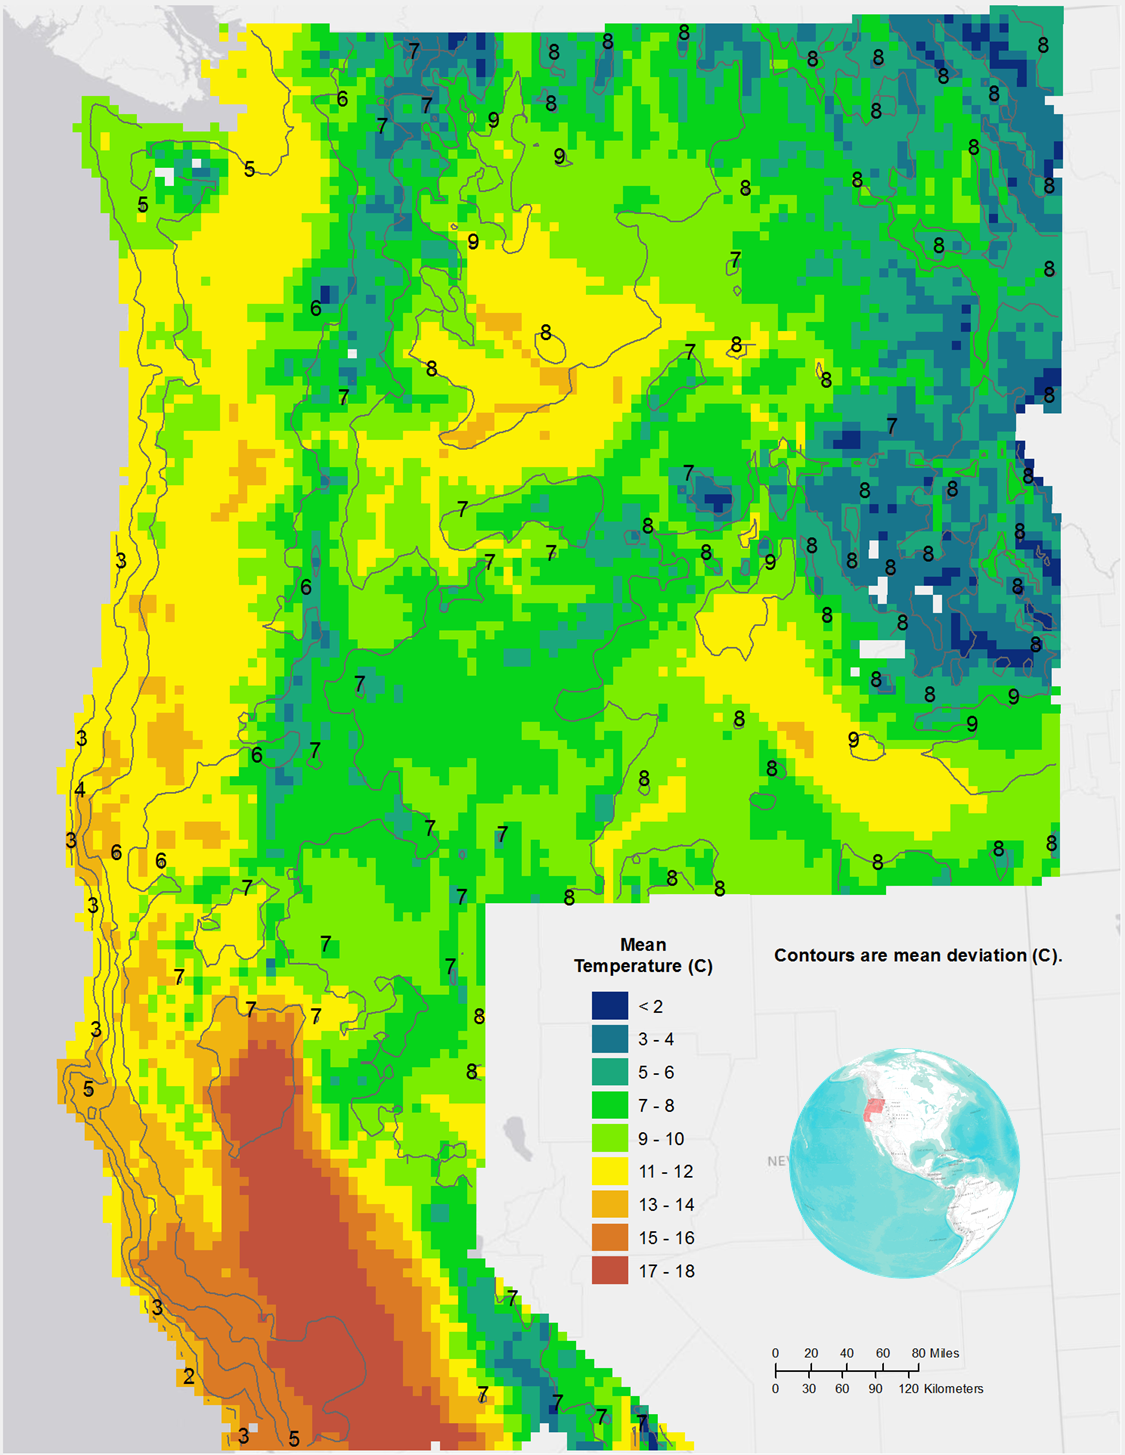
\includegraphics[width=1\linewidth]{temp}  
\caption{Mean annual temperature, with isolines showing the standard deviation in monthly temperature.}
  \label{fig:temp}
\end{figure}

\begin{figure}[hp]
  \centering  
  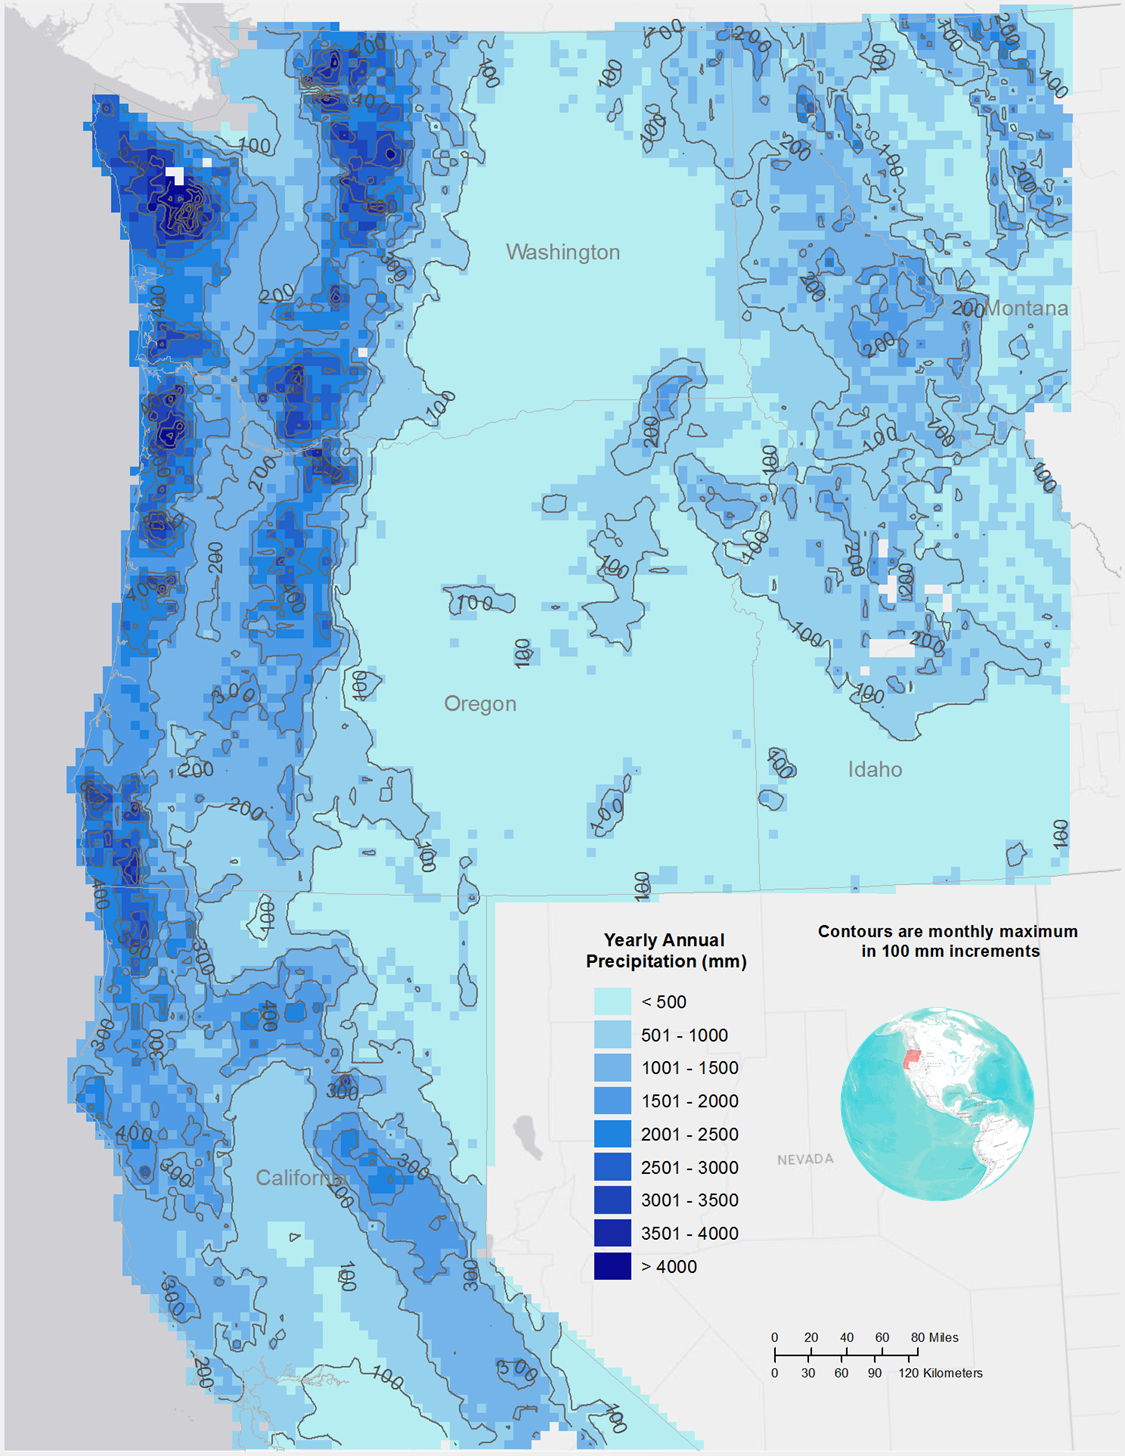
\includegraphics[width=1.0\linewidth]{precip}  
\caption{Total annual precipitation, with isolines showing the maximum monthly precipitation.}
  \label{fig:precip}
\end{figure}

In order to determine incoming monthly solar radiation, monthly
\acf{NREL} global incident radiation data were
utilized ~\cite{Perez2002}.  The incident radiation data product
provides monthly average and annual average daily total solar resource
averaged over surface cells of 0.1 degrees.  Hourly radiance images
from geostationary weather satellites, daily snow cover data, and
monthly averages of atmospheric water vapor, trace gases, aerosols are
used to calculate the hourly total direct and diffuse insolation
falling on a horizontal surface.  Existing ground measurement stations
validate the data where available. Where no existing ground weather
stations exist, the model is assumed to be the best estimate.

The incident radiation data is available as a grid with a scale
similar to this project and is interpolated (cubic-spline) onto the
\ac{AHB} pixels.

\subsubsection{Soil Parameters}
\label{sec:soil}

\ac{3pg} uses a single layer soil model that maintains an estimate of
the amount of water available at any timestep in the model.  In
addition, \ac{3pg} includes a growth limiter related to the available
water in the soil, and the soil type.

These soil parameters are determined with the \acf{STATSGO}
database~\cite{STATSGO}.  \ac{STATSGO} is a national soil database,
distributed by the \ac{NRCS}.  \ac{STATSGO} maps are designed for
regional studies, and the soil inventories are typically generalized
from more detailed surveys, or from a combination of ancillary
datasets.  Individual \ac{STATSGO} areas can contain multiple soil
components, and the map units are linked to attributes the soil data
base which gives the proportionate extent of the component soils and
their associated properties.  The \ac{mmu} is about 625 (ha).  For
each pixel in the modeling grid, intersecting map units are averaged
for the estimated pixel values.  1887 different soil delineations were
used, contributing anywhere from 144 to 1.3M (ha).

\ac{maxAWS} defines the holding capacity of the soil.
\ac{maxAWS} is directly taken from the \ac{STATSGO} database which
determines the maximum water holding capacity through the complete
horizon over the topmost 1 (m) of soil (Figure~\ref{fig:aws}).

\begin{figure}
  \centering
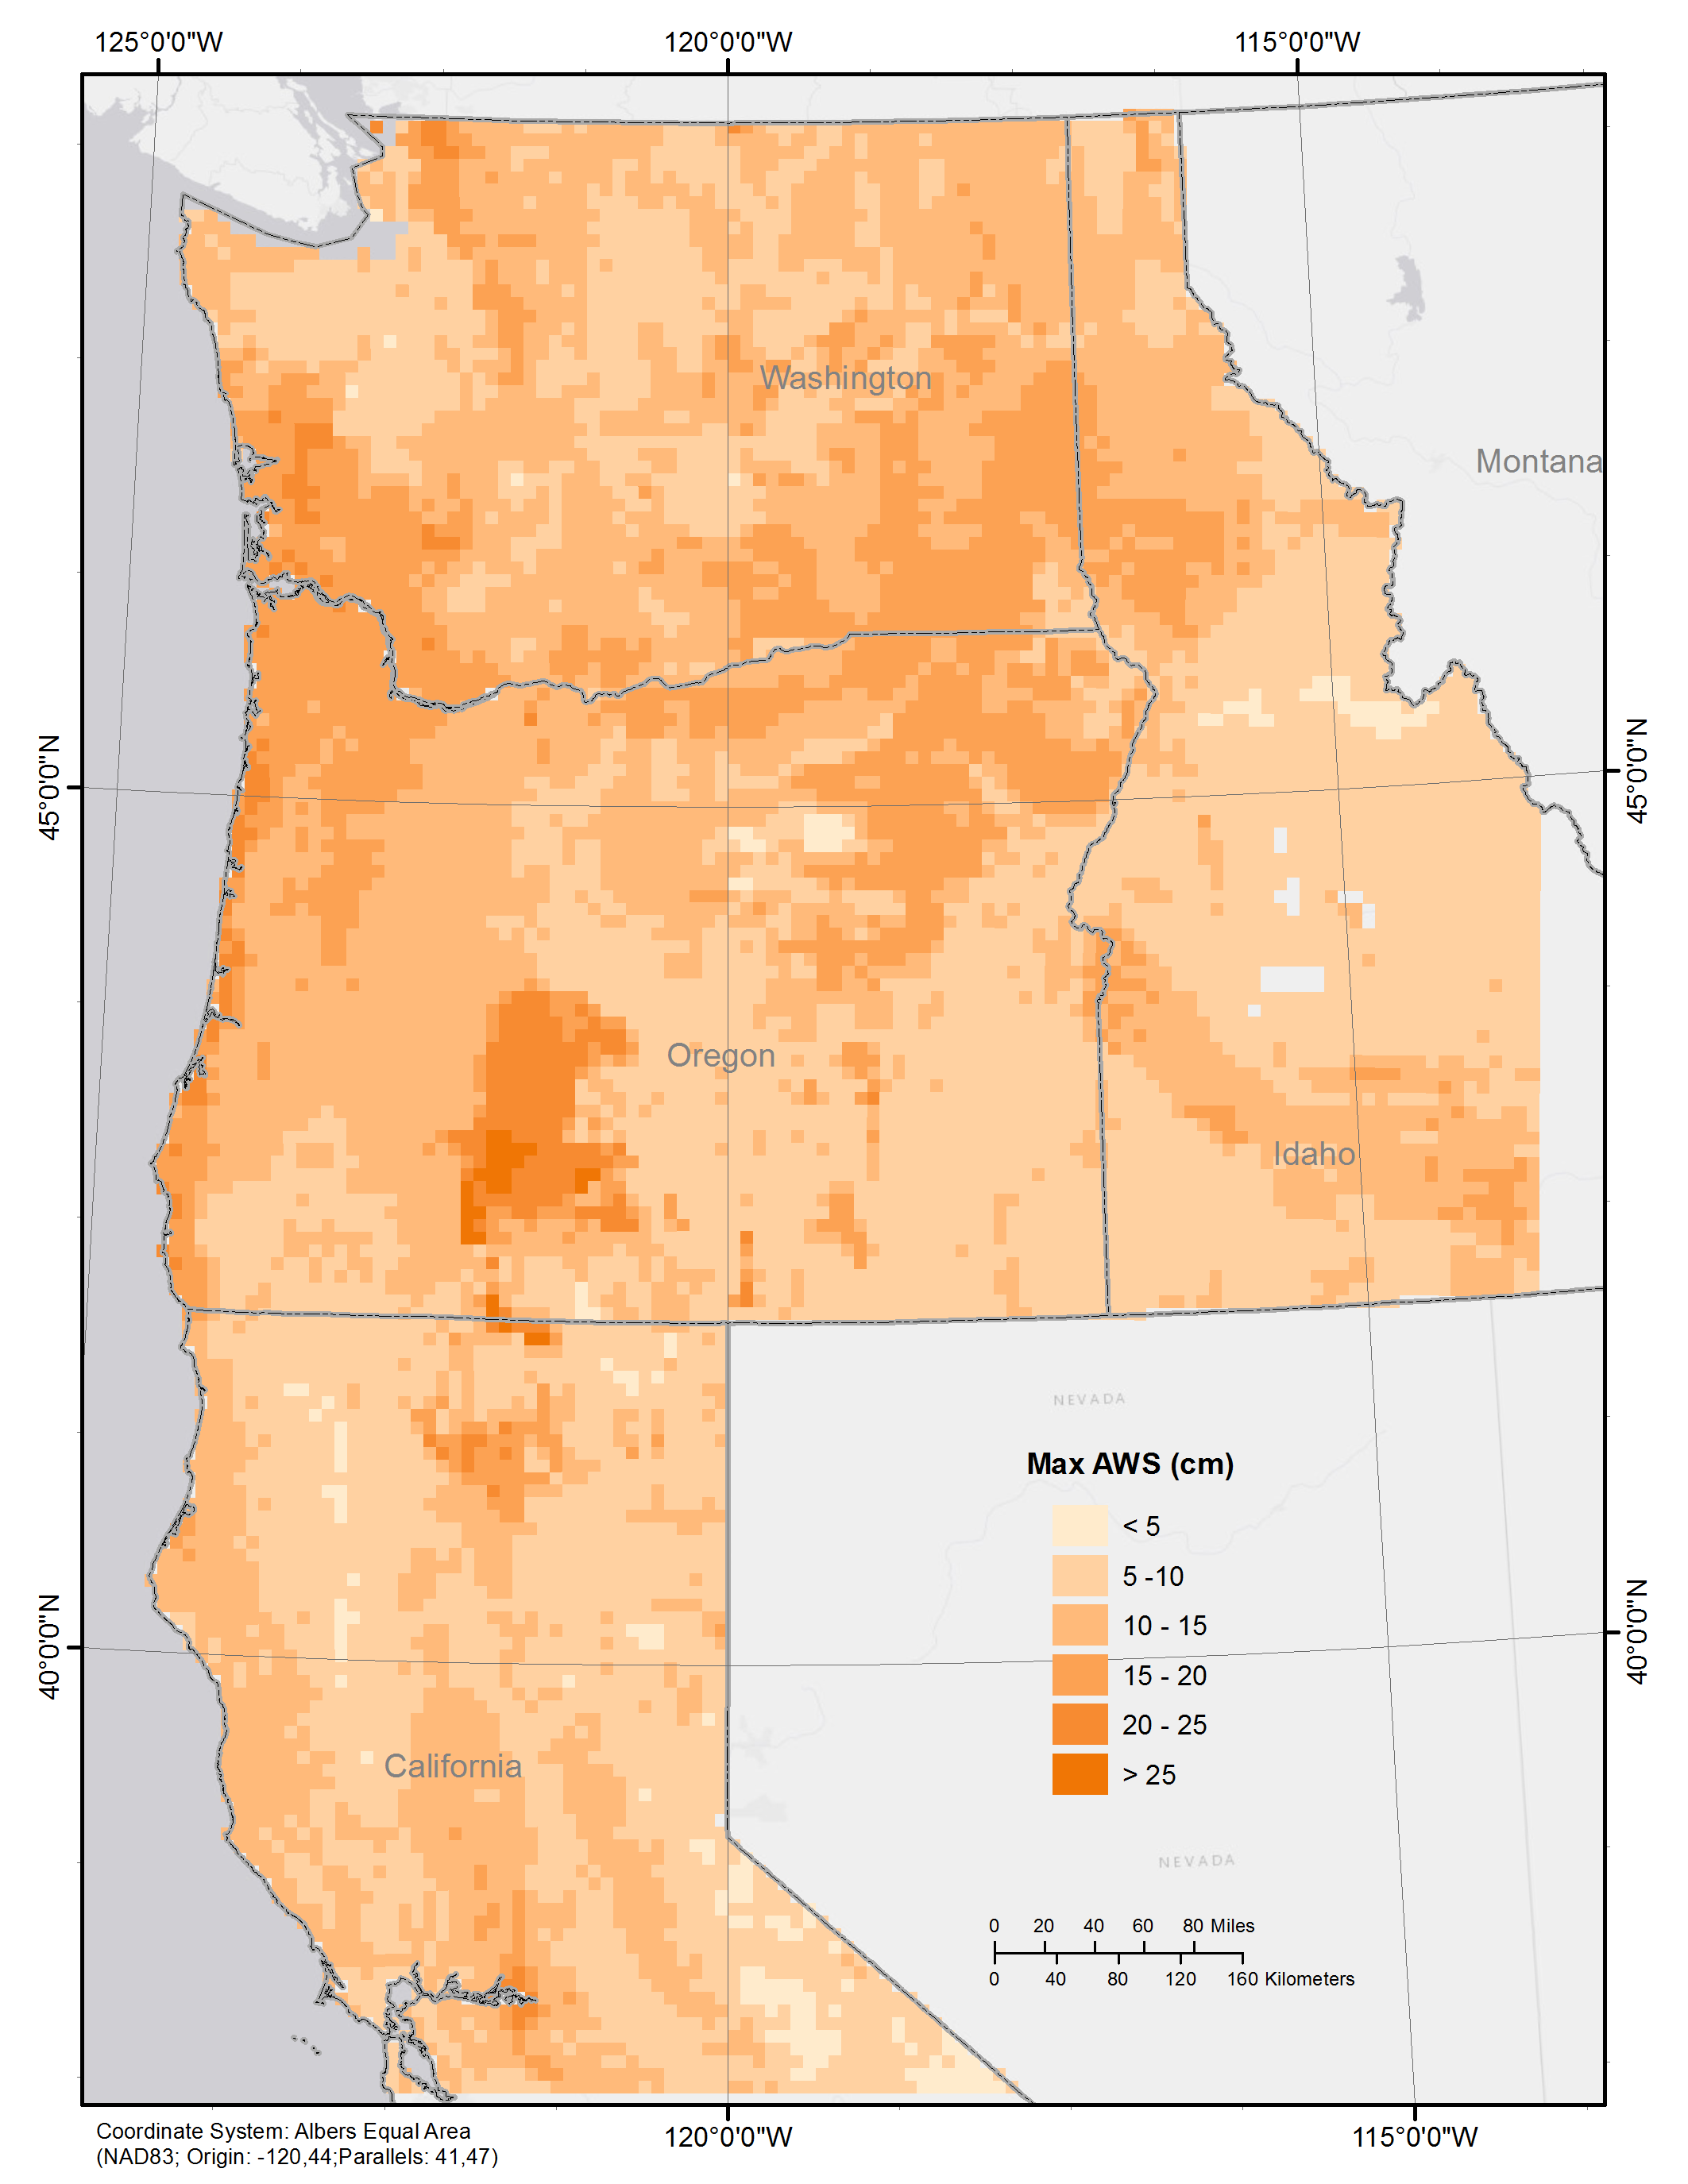
\includegraphics[width=1\linewidth]{maxaws}
  \caption{\ac{STATSGO} derived maximum water holding capacity.}
  \label{fig:aws}
\end{figure}

The \ac{fSW} is parameterized with a power \acs{swp} and a constant
\acs{swc}, both functions of the soil type
(Figure~\ref{fig:soil-triangle}).  The soil type is determined from
\ac{STATSGO} report percentages of silt, sand, and clay within each
soil component.

%\begin{equation*}
%\acs{fSW} = \frac{1-(1-\acs{AWS}/\acs{maxAWS})^{\acs{swp}}}{1+((1-\acs{AWS}/\acs{maxAWS})/\acs{swc})^{\acs{swp}}}
%\end{equation*} 

\begin{figure}
  \centering
  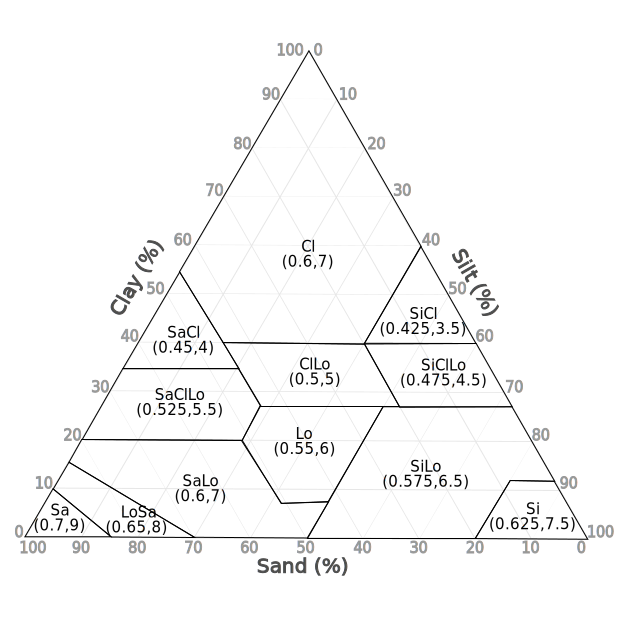
\includegraphics[width=0.52\linewidth]{soil_triangle}
    \begin{tikzpicture}
    \begin{axis}[
      name=fsw,
      xmin=0,xmax=1,
      xtick={0,.2,.4,.6,.8,1},
      xticklabels={0,.2,.4,.6,.8,1},
      xlabel=$\acs{AWS}/\acs{maxAWS}$,
      ymin=0,ymax=1,
      ytick={0,.2,.4,.6,.8,1},
      yticklabels={0,.2,.4,.6,.8,1},
      ylabel=$\acs{fSW}$,
      no markers,
      width=0.45\linewidth,
      height=0.45\linewidth,
      every axis plot/.append style={line width=1pt},
      legend entries={sand,clay,silt},
      legend style={
        at={(0.5,1.0)},anchor=south,legend columns=-1,yshift=2pt}
      ]
      \addplot+[color=red] table [x=awsp, y=Sand, col sep=comma] {soil-fsw.csv};
      \addplot+[color=orange] table [x=awsp, y=Clay, col sep=comma] {soil-fsw.csv};
      \addplot+[color=green] table [x=awsp, y=Silt, col sep=comma] {soil-fsw.csv};
    \end{axis}
  \end{tikzpicture}

  \caption{(\acs{swc},\acs{swp}) pairs as determined by soil
    composition.  Included is a graph for the function $\acs{fSW} =
    \frac{1-(1-\acs{AWS}/\acs{maxAWS})^{\acs{swp}}}{1+((1-\acs{AWS}/\acs{maxAWS})/\acs{swc})^{\acs{swp}}}$
    for sand,silt and clay. }
  \label{fig:soil-triangle}
\end{figure}

\subsection{Land Classification and Irrigation}
\label{sec:land}

Available climatic data makes it possible to make estimations for
poplar growth throughout the \ac{PNW} region.  This may provide
interesting comparisons of changes in yield, but is not suitable
for determining regional estimations, as not all lands are equally likely
to be available for poplar plantations.  Variables like land
ownership, topography and salinity, influence the technical capability
of growing poplar.  

In addition, the ability to irrigate a poplar plantation can have
large effects on the predicted yields of poplar.  Determining which
areas in the \ac{PNW} region are liable to be available for irrigation
can significantly influence regional poplar harvest estimations.  

To limit the areas within the \ac{PNW} region to areas that are
technically suitable to poplar plantations, a set of masks were used.
Permanently non-suitable land was removed from consideration. Lands
under Federal ownership~\cite{NationalAtlasoftheUnitedStates2013} and
currently developed land were excluded from consideration.  Physical
features including slopes greater than 15\%~\cite{Gesch2007}, and soil
salinity greater than 4 ($dS/m$) were also
excluded.

%The land suitability study included other factors for poplar
%suitability; nine variables considered important for poplar growth
%were identified: growing season precipitation, temperature, and
%length; soil texture and drainage, pH, salinity, and depth; water
%table depth; and slope.  Most of these parameters are included more
%explicitly in the \ac{3pg} model, and directly affect yield
%predictions.  Soil salinity and pH have not yet been integrated into
%the \ac{3pg} model.

% References FAO. 1976. FAO A framework for land evaluation. Soils Bulletin 32. Food and Agriculture Organization of the United Nations, Rome (1976).

Available water for irrigation is an important question when dealing
with crops in the \ac{PNW}.  Irrigation is a combination of
availability and rights, that is hard to track on a regional scale.
However, one aspect of irrigation is that if it's available it is
likely being used.  Therefore, for determining irrigated yield
predictions for poplar, a mask of existing irrigated agricultural
areas was used.  These locations were determined in two steps.  First,
the a cropland data layer was used to spatially locate agricultural
crops in the region.  The USDA, NASS Cropland Data Layer (CDL) is a
nationally available raster of crop specific land cover data layer
with a ground resolution of 30 meters.  The CDL is produced using
satellite imagery with a classification emphasis on agricultural land
cover~\cite{Boryan2011a}.  The CDL was projected unto the \ac{AHB}
region.  Individual pixels from the CDL were then aggregated within
the larger model's pixels to determine fractional composition of each
pixel~(Figure~\ref{fig:land}).  An additional step was used to adjust
the total area in each county to the values of hectares reported to
the \ac{NASS}.  \ac{NASS} publishes U.S., State and County
agricultural statistics for many commodities~\cite{Service2015}.
Later modeling efforts rely on the \ac{NASS} reported hectares of the
various commodities harvested.  This was accomplished by uniformly
adjusting the CDL derived pixel fractions, so that sum of pixel
fractions over any county in the \ac{AHB} region match the reported
number of hectares harvested for that county and commodity.  This
method allows the spatial patterns of the CDL to be retained with
fractions that add to the \ac{NASS} reported values.

All images were scaled to match the $\approx$64 km\textsuperscript{2}
project pixel resolution. Scaled pixels reflect the area weighted
average of any smaller pixels.

\begin{figure}[hp]
  \centering
% https://docs.google.com/drawings/d/1oadbCuHL61duRoK8jAAtMSCu3bQYRyvM43AaDtOwpzw/edit?usp=sharing
  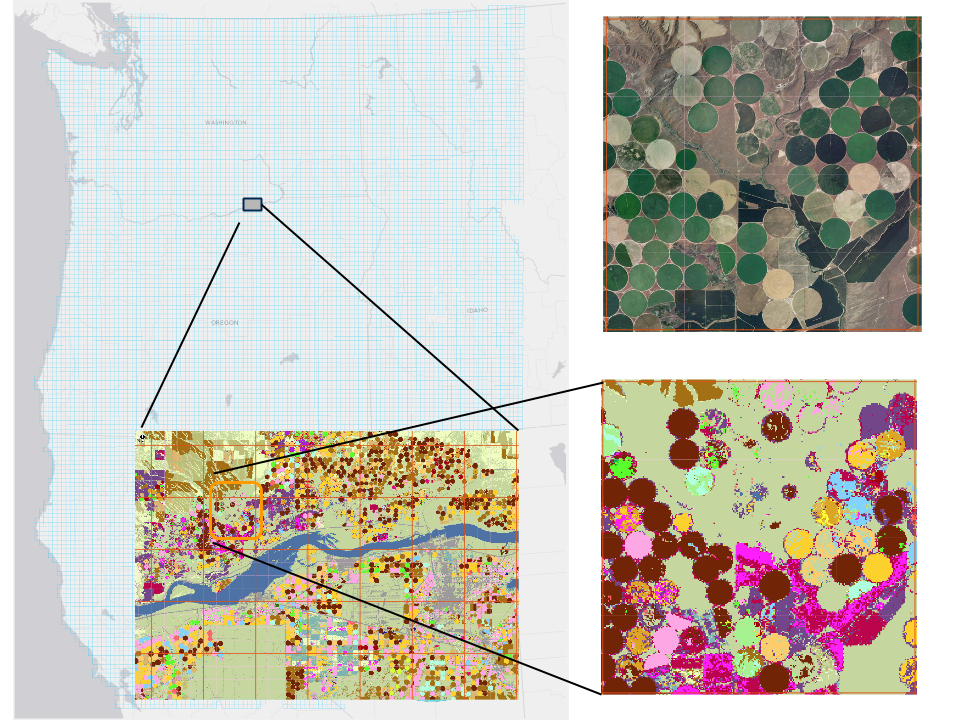
\includegraphics[width=1\linewidth]{land.png}
  \caption{Agricultural Land Classification.  Each \ac{AHB} pixel is made up of
    many remotely sensed derived \ac{CDL} crop classifications.  This
    are aggregated to determine fractional amount of coverage for each
    \ac{AHB} pixel. }
  \label{fig:land}
\end{figure}

\subsection{Climate Change}

The A1B climate change scenario
articulated in the \ac{IPCC} 2007 Summary for Policymakers is
plausible, somewhat optimistic
scenario for climate change~\cite{IPCC2007,Parry2007}. The A1B scenario predicts a balanced utilization of available energy
sources, with similar improvement rates applied to all energy supply
and end-use.  The future is one of rapid economic growth, global
population that peaks in mid-century and declines thereafter, and a
rapid introduction of new and more efficient
technologies. 

We used expected conditions based on the A1B
scenario to demonstrate the effect of potential climate change on yield
predictions in the near future. Yields were predicted based A1B scenario outcomes on a
plantation initiated in 2040.

Estimations of the expected change in temperature and precipitation were derived from the \ac{CCSM3}.  The \ac{CCSM3} is a climate model
with components including the atmosphere, ocean, sea ice, and land
surface. \ac{CCSM3} is designed to produce realistic simulations over
a wide range of spatial and temporal resolutions.  \ac{CCSM3}
predictions are available at 0.5 degree grid cells.  Estimations of
change in the next fifty years were used in these climate change
estimations.

The \ac{CCSM3} estimations cannot be used directly, especially
comparatively to the current estimations using the \ac{PRISM} data.
This is because when comparing the \ac{CCSM3}'s somewhat coarse scale
estimations to the more detailed \ac{PRISM} estimations the current
(2000-2014) predictions exhibit bias.  Therefore, the \ac{CCSM3}
estimations were used to determine the predicted change in temperature
and precipitation for the \ac {AHB} region, and these changes were
then applied to the current \ac{PRISM} estimations. For example, the
40 year change in temperature, and precipitation for the A1B scenario
shows a mean increase in temperature of about 1\degree Celsius, with
larger changes in the South and West.  Mean annual precipitation
decreases by about 100 (mm) throughout the region with larger changes
in along the coast~(Figure~\ref{fig:change}).

\begin{figure}[hp]
  \centering
  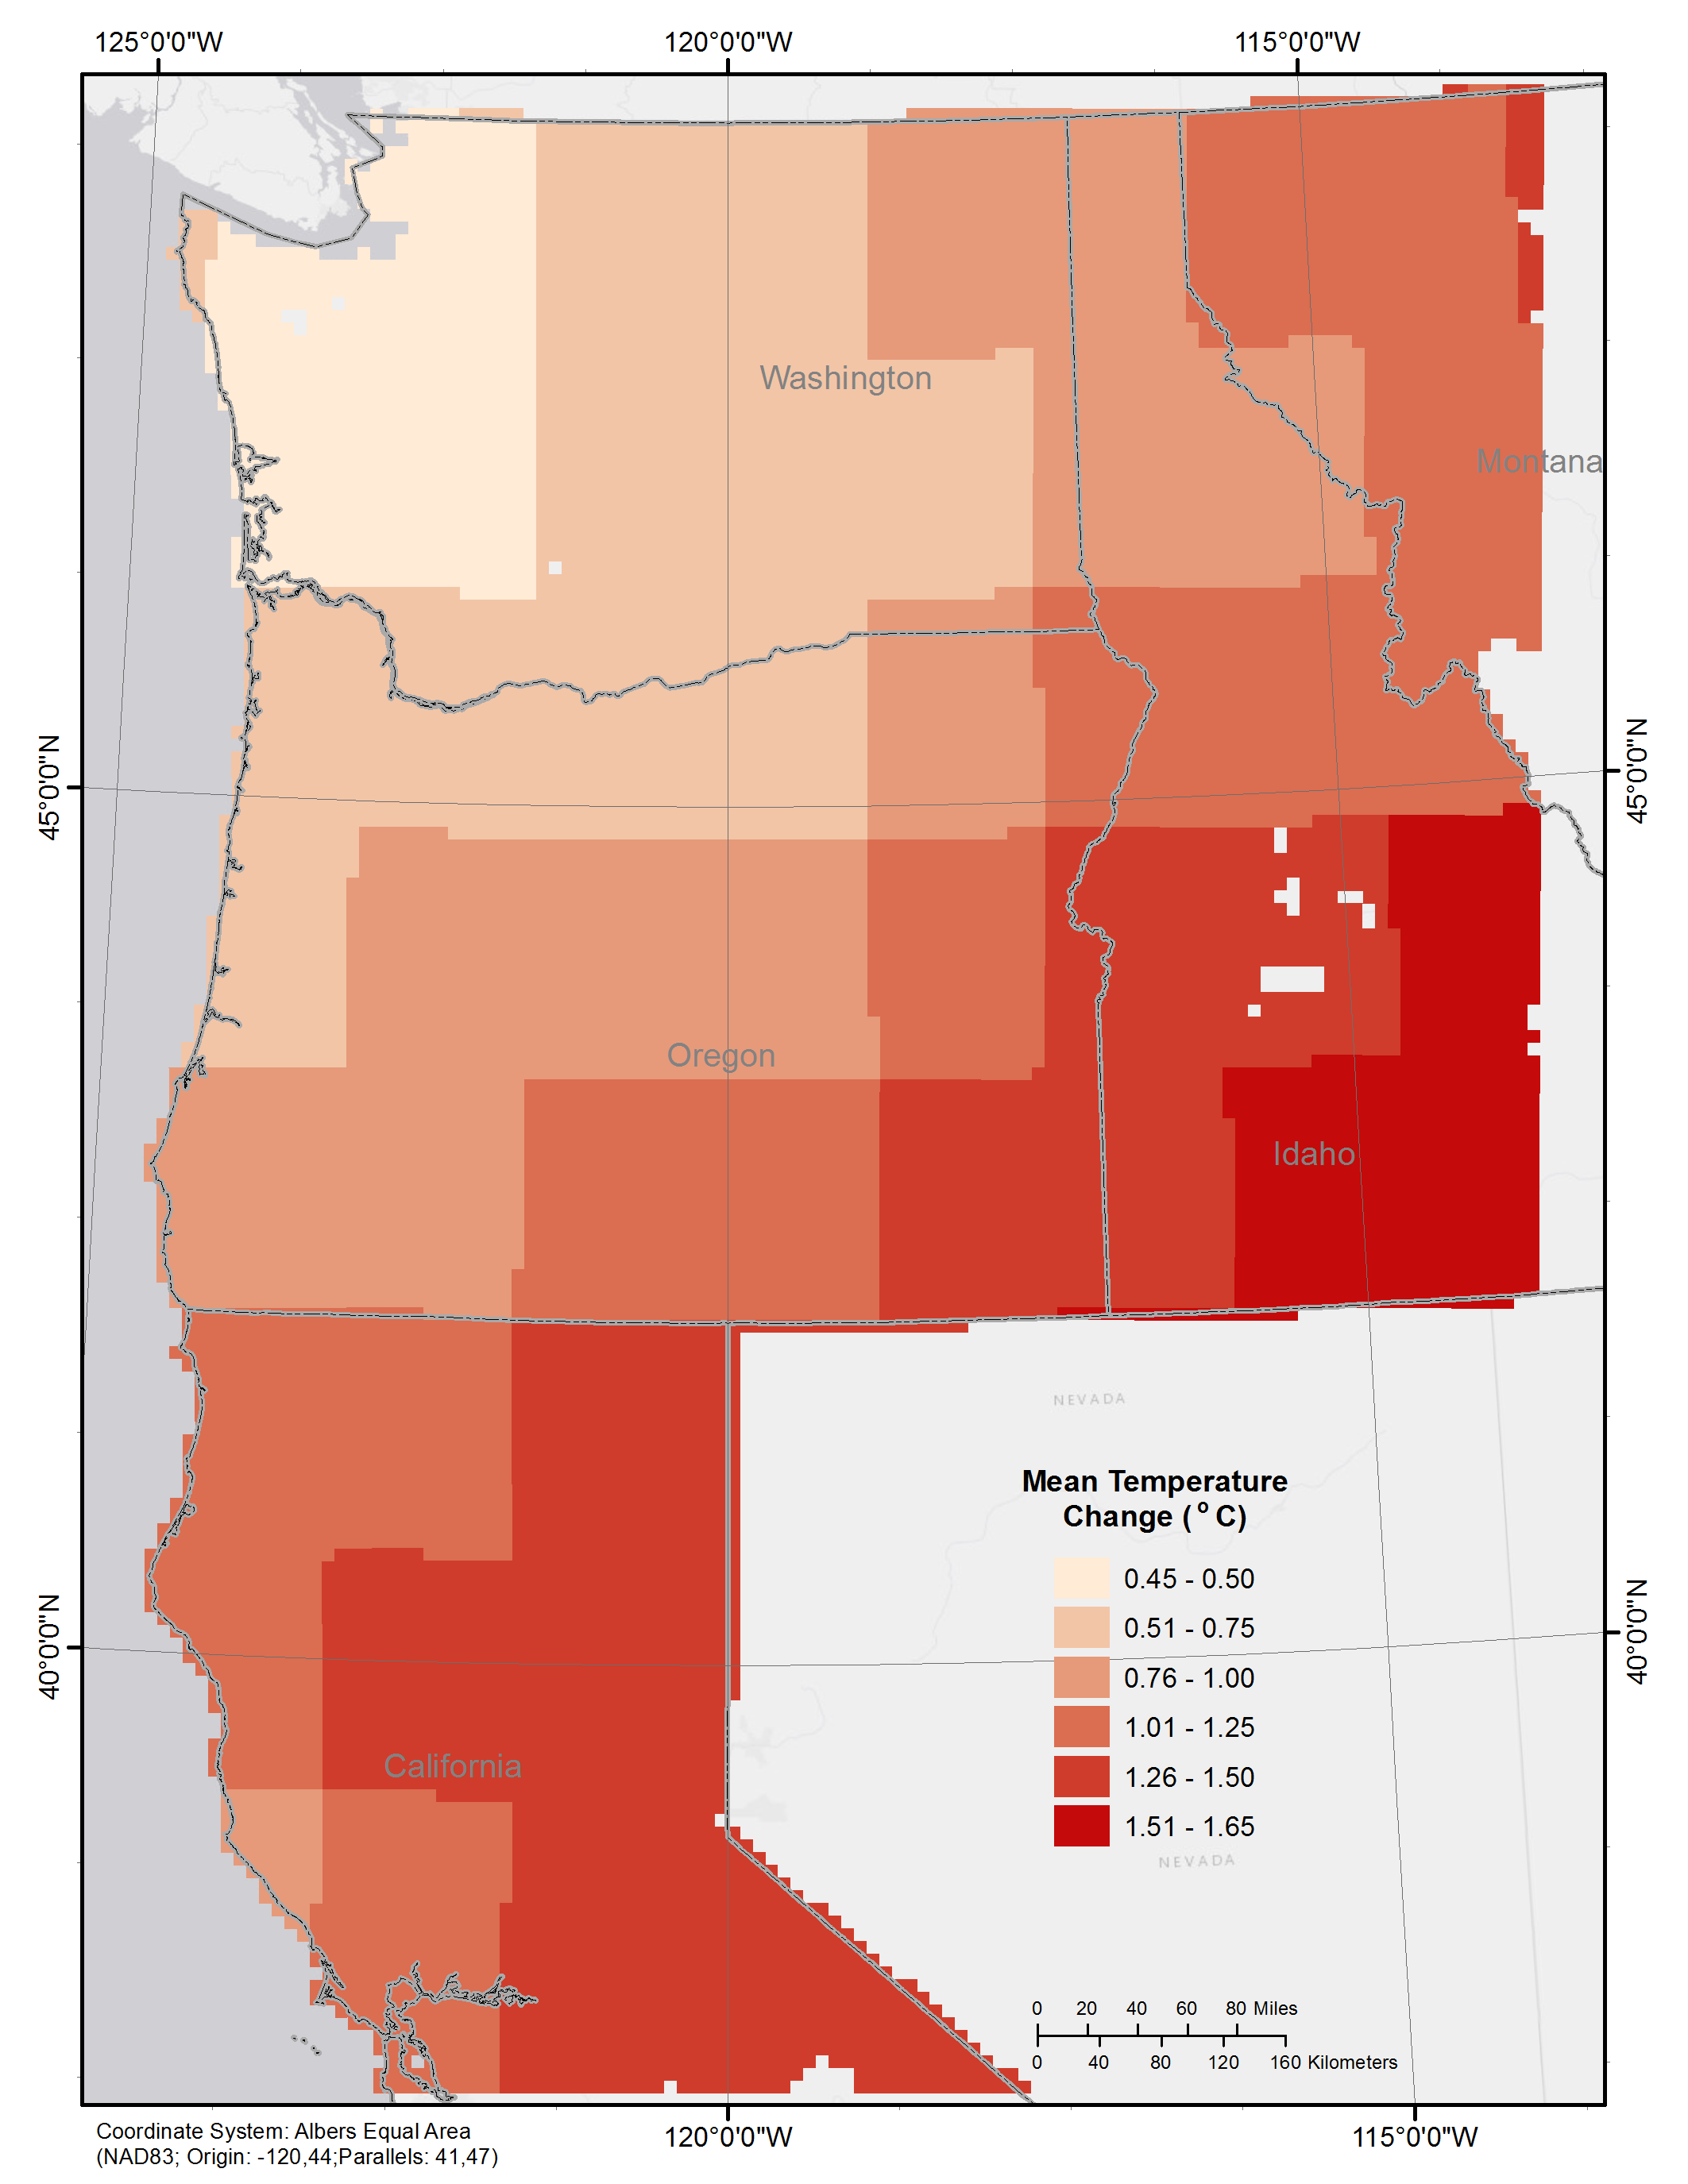
\includegraphics[width=0.45\linewidth]{temp_change}
  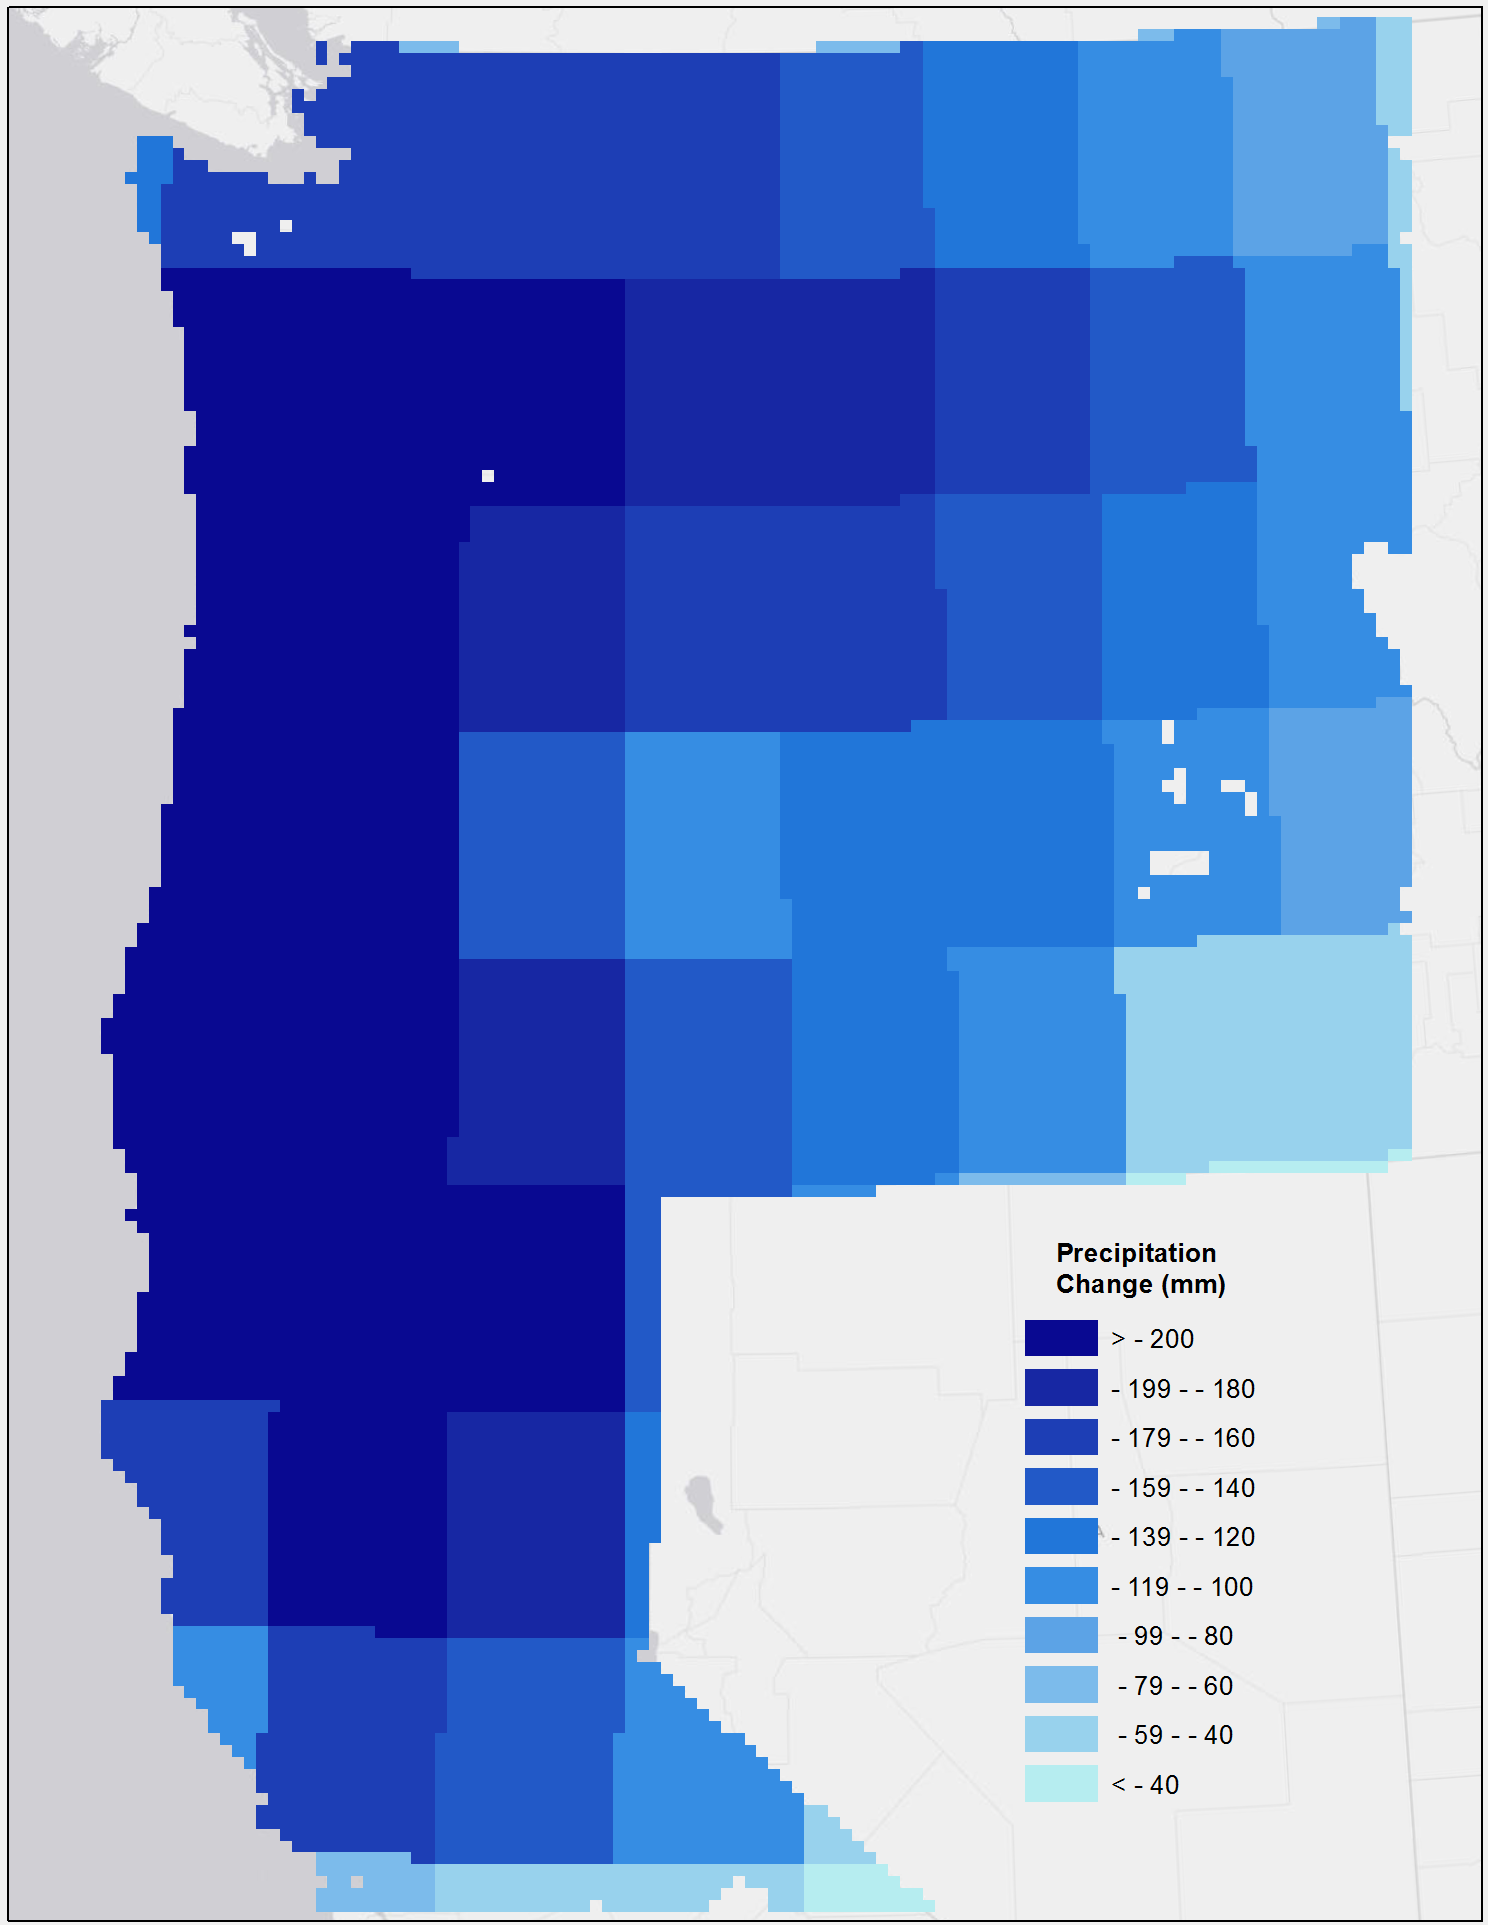
\includegraphics[width=0.45\linewidth]{precip_change.png}
  \caption{Predicted changes in temperature and precipitation under \ac{CCSM3} scenario A1B for plantation planted in 2040.}
  \label{fig:change}
\end{figure}

\section{Results and Discussion}

Results show an average coppice yield for irrigated poplar over the
entire region of 19.7 (Mg/ha).  38000 ($km^2$) were included in the
estimate.  Yields were highest in the central valley of California, a
rich agricultural center, with similar yields along the temperate
western parts of Oregon and Washington.  Yields decreased in eastern
Washington, reaching lows in the Northeastern section of the study
region~(Figure~\ref{fig:irrigated_yield}).

\begin{figure}[hp]
  \centering
  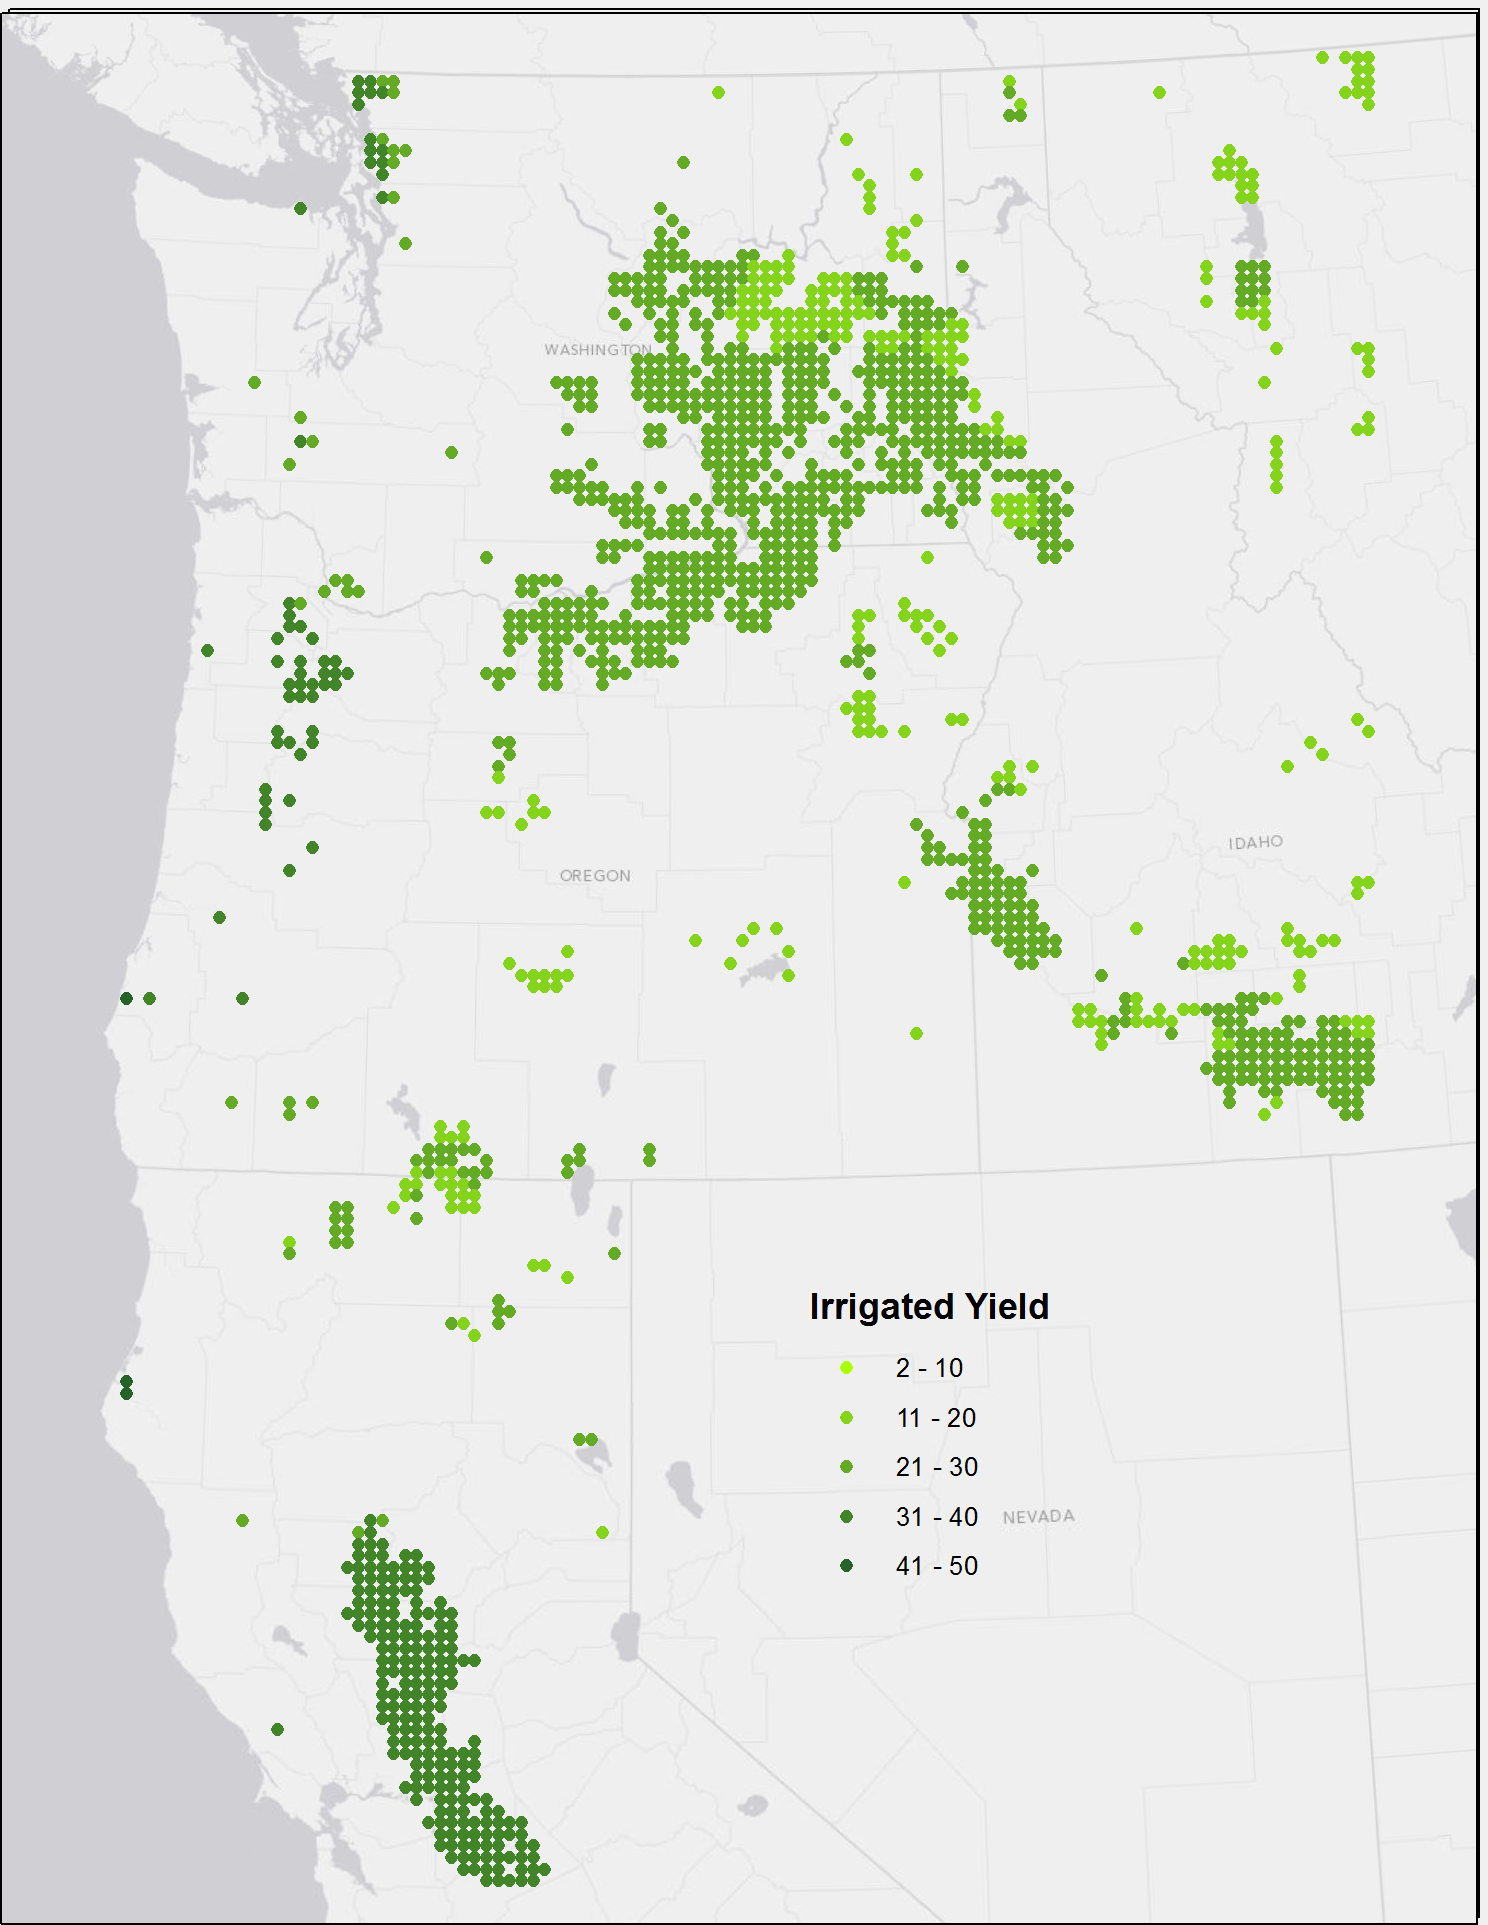
\includegraphics[width=1.0\linewidth]{irrigated_yield}
  \caption{Predicted irrigated yield of a 3 year coppice harvest for
    areas under agricultural practice.  The image only
    includes pixels with more that \%20 area identified as cropland.}
  \label{fig:irrigated_yield}
\end{figure}

Similarly, the non-irrigated yield predictions were masked with the
areas excluded in the land suitability study to include those areas
likely to support non-irrigated poplar plantations.  Results for the
non-irrigated lands predict an average coppice yield of 6.6 (Mg/ha)
over an area under consideration of 57000 ($km^2$).  In the case of
non-irrigated yields, the highest yields were along the Pacific coast
where precipitation is most plentiful, and more uniform in the inland
areas of the \ac{AHB} region~(Figure~\ref{fig:nonirrigated_yield}).

\begin{figure}[hp]
  \centering
  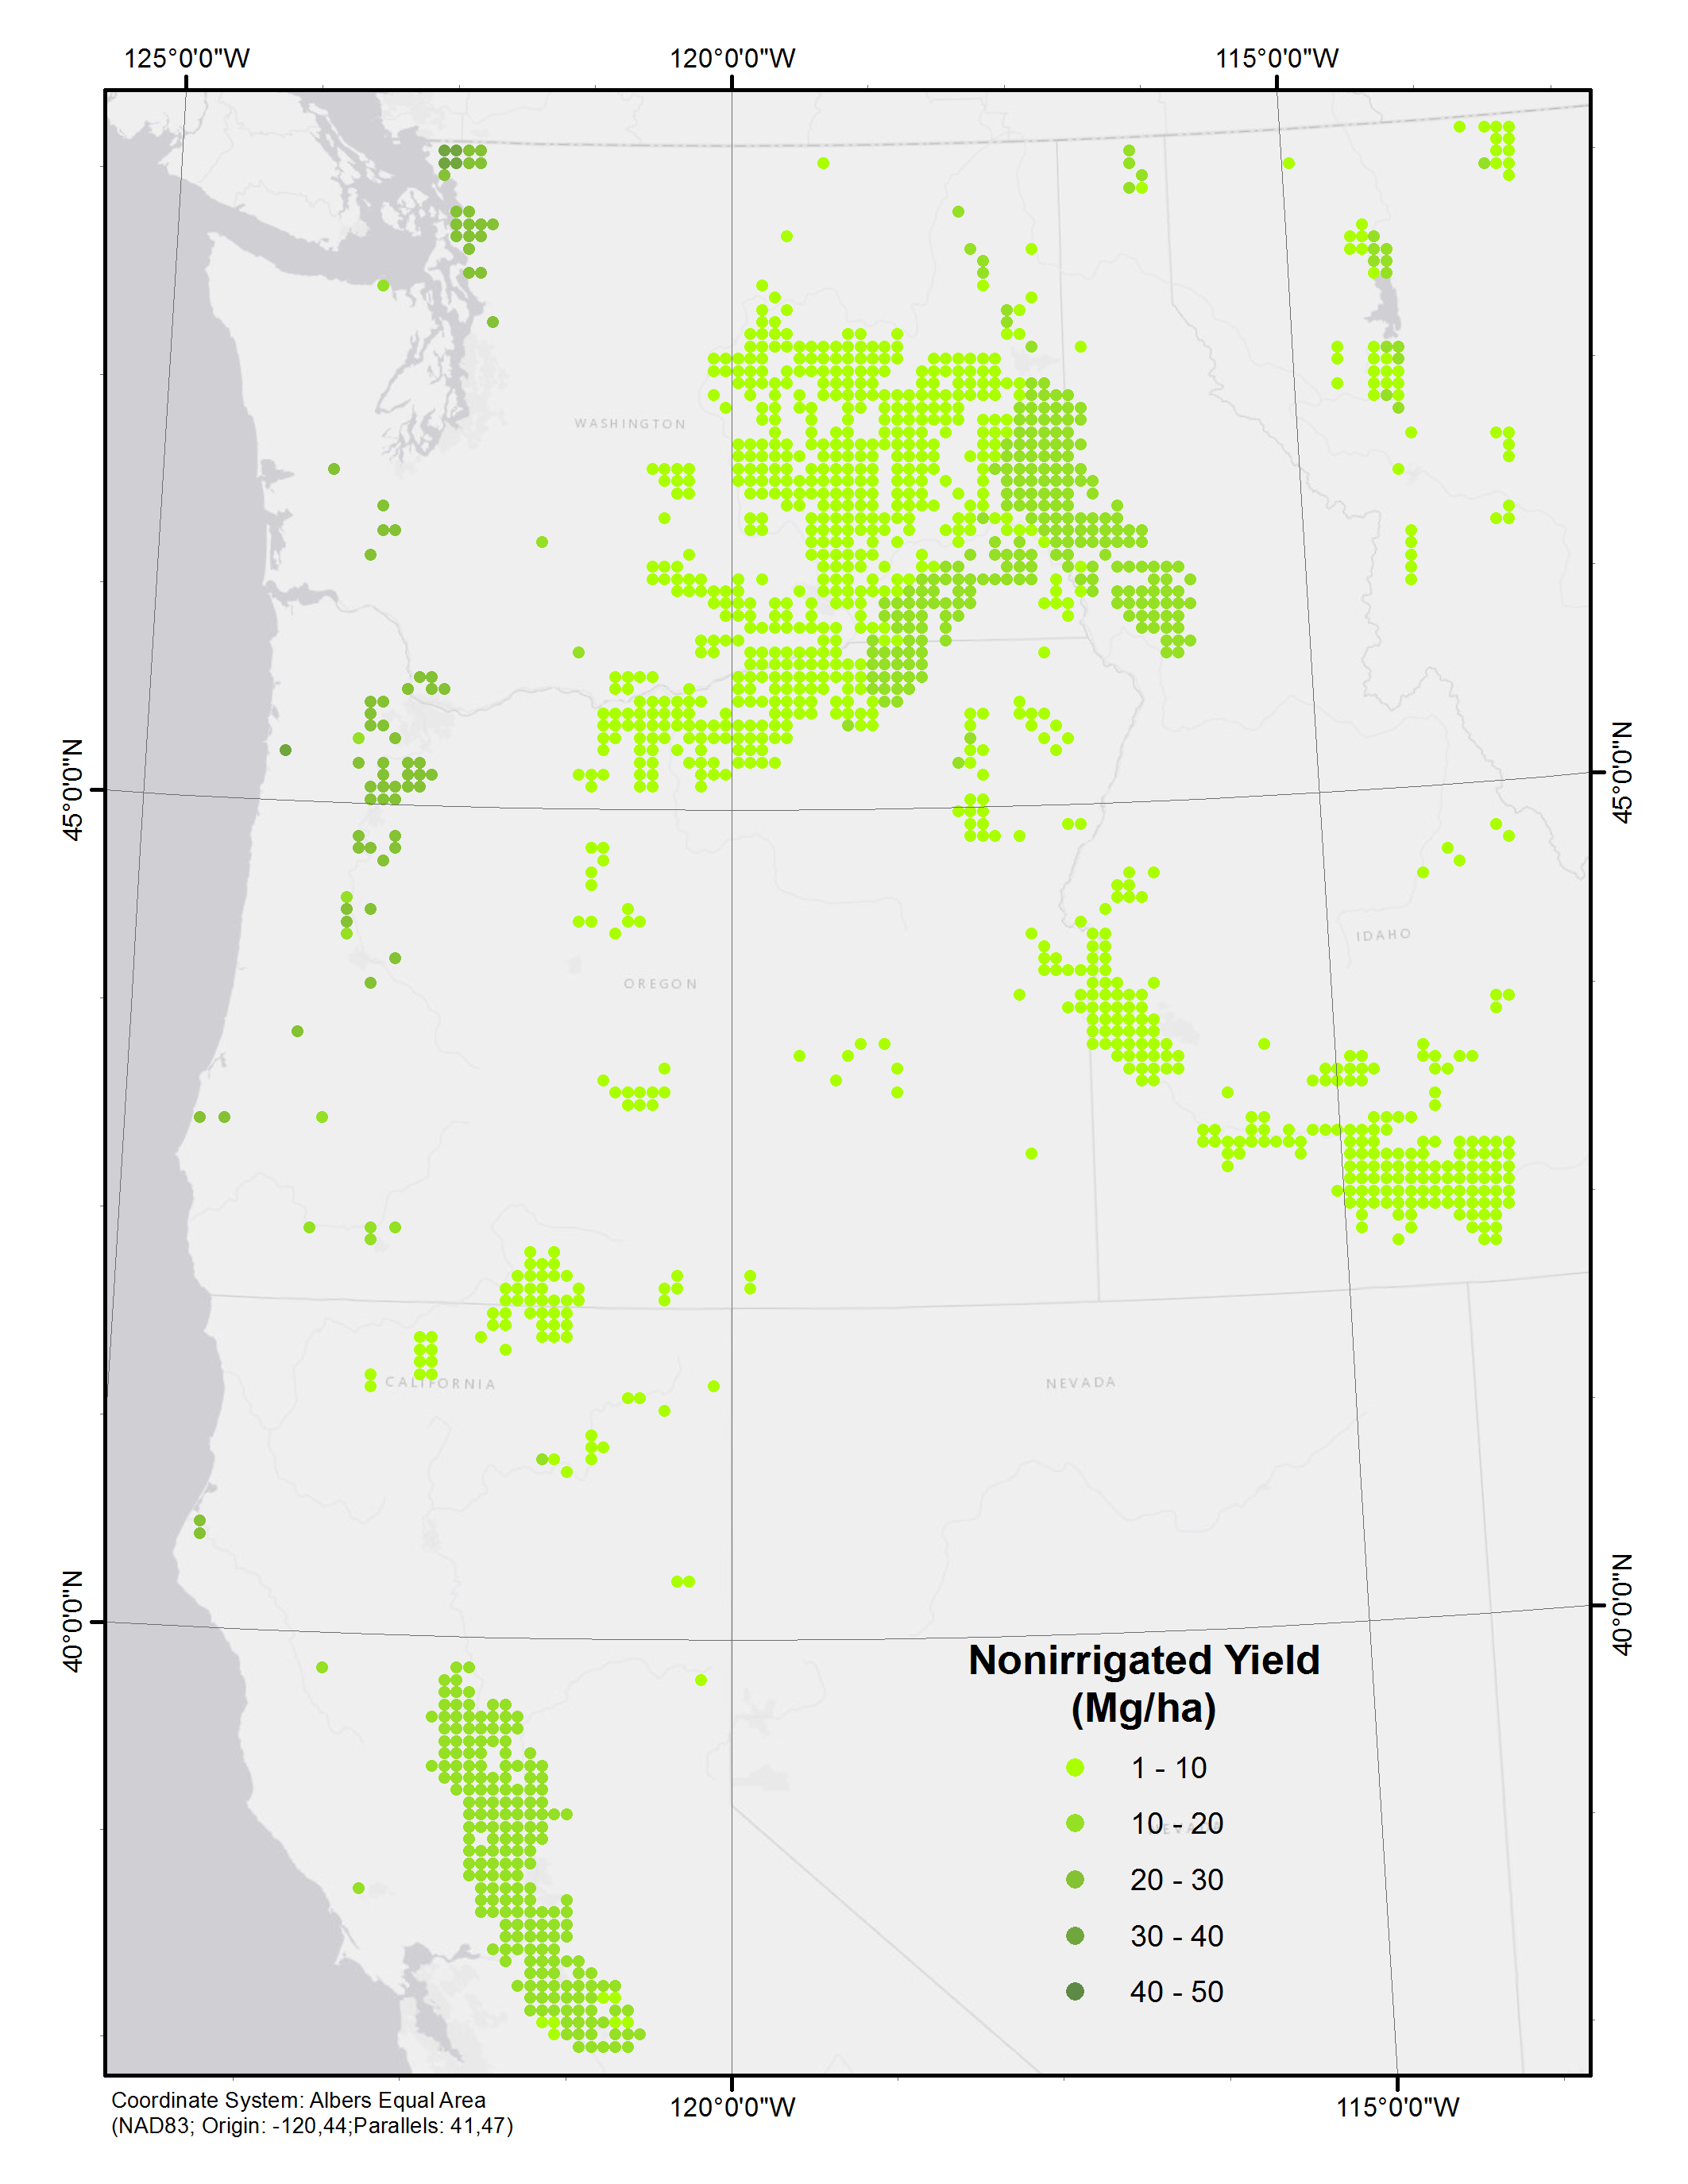
\includegraphics[width=1.0\linewidth]{nonirrigated_yield}
  \caption{Predicted non-irrigated yields of a 3 year coppice
    harvest for areas identified as rangeland or marginal land.  The
    image only includes pixels with areas more than \%20.}
  \label{fig:nonirrigated_yield}
\end{figure}

To assess the predicted change in yields from the A1B example study,
the model was rerun
with the predicted changes in temperature and precipitation.  The
results were averaged and summarized as above to predict yields.  The
yields were then compared to the current yield estimates to determine
the difference in predicted yields under that one example climate
change scenario.

Under irrigated conditions, the higher predicted temperatures
generally improve yields through most of the region, with the
exception of California, where high temperatures often limit monthly
growth.  Changes in yield are modest in the areas with the highest
yields and more significant in the colder northern and central
regions~(Figure~\ref{fig:new_irrigated}).
 
\begin{figure}[hp]
  \centering
  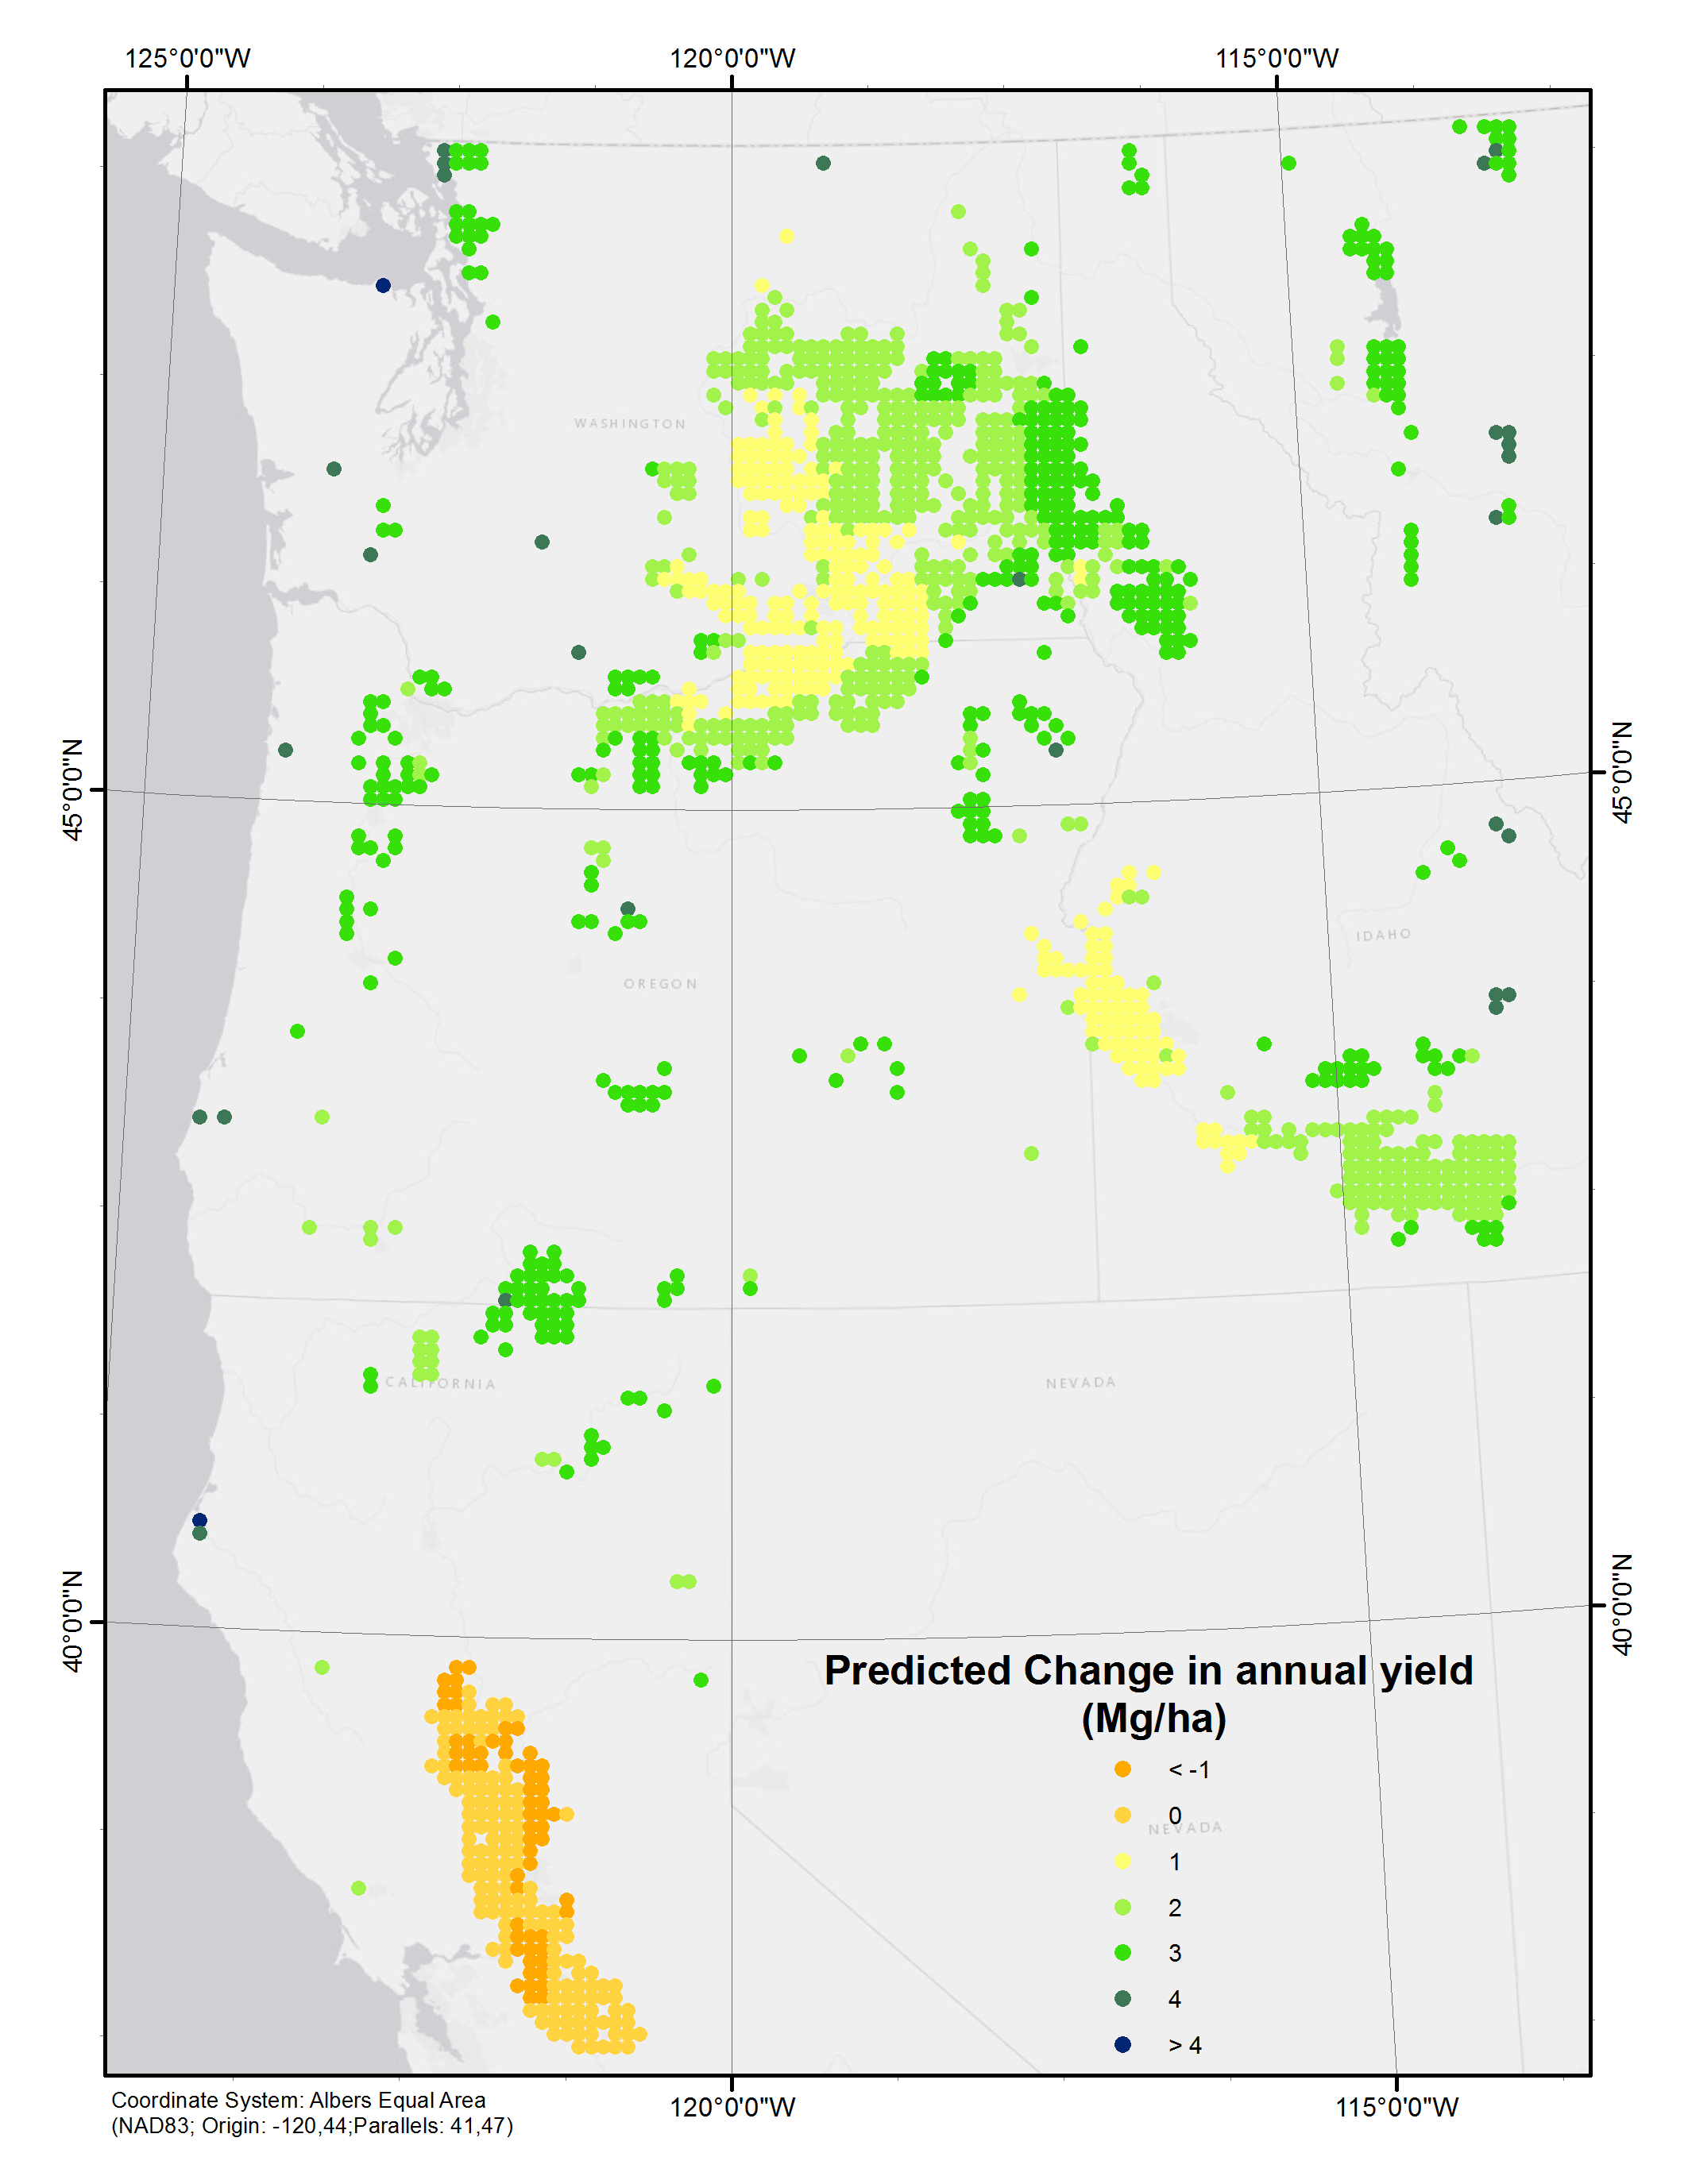
\includegraphics[width=1\linewidth]{climate_irrigated}
  \caption{Changes in predicted irrigated yield for \ac{CCSM3} scenario A1B
    for a plantation planting in 2040-2058.}
  \label{fig:new_irrigated}
\end{figure}

For non-irrigated plantations, the predicted decrease in precipitation
decreases yields along the areas with the current highest yields,
along the wet Pacific coast.  Higher temperatures continue to increase
yields in most of the inland areas~(Figure~\ref{fig:new_nonirrigated})

\begin{figure}[hp]
  \centering
  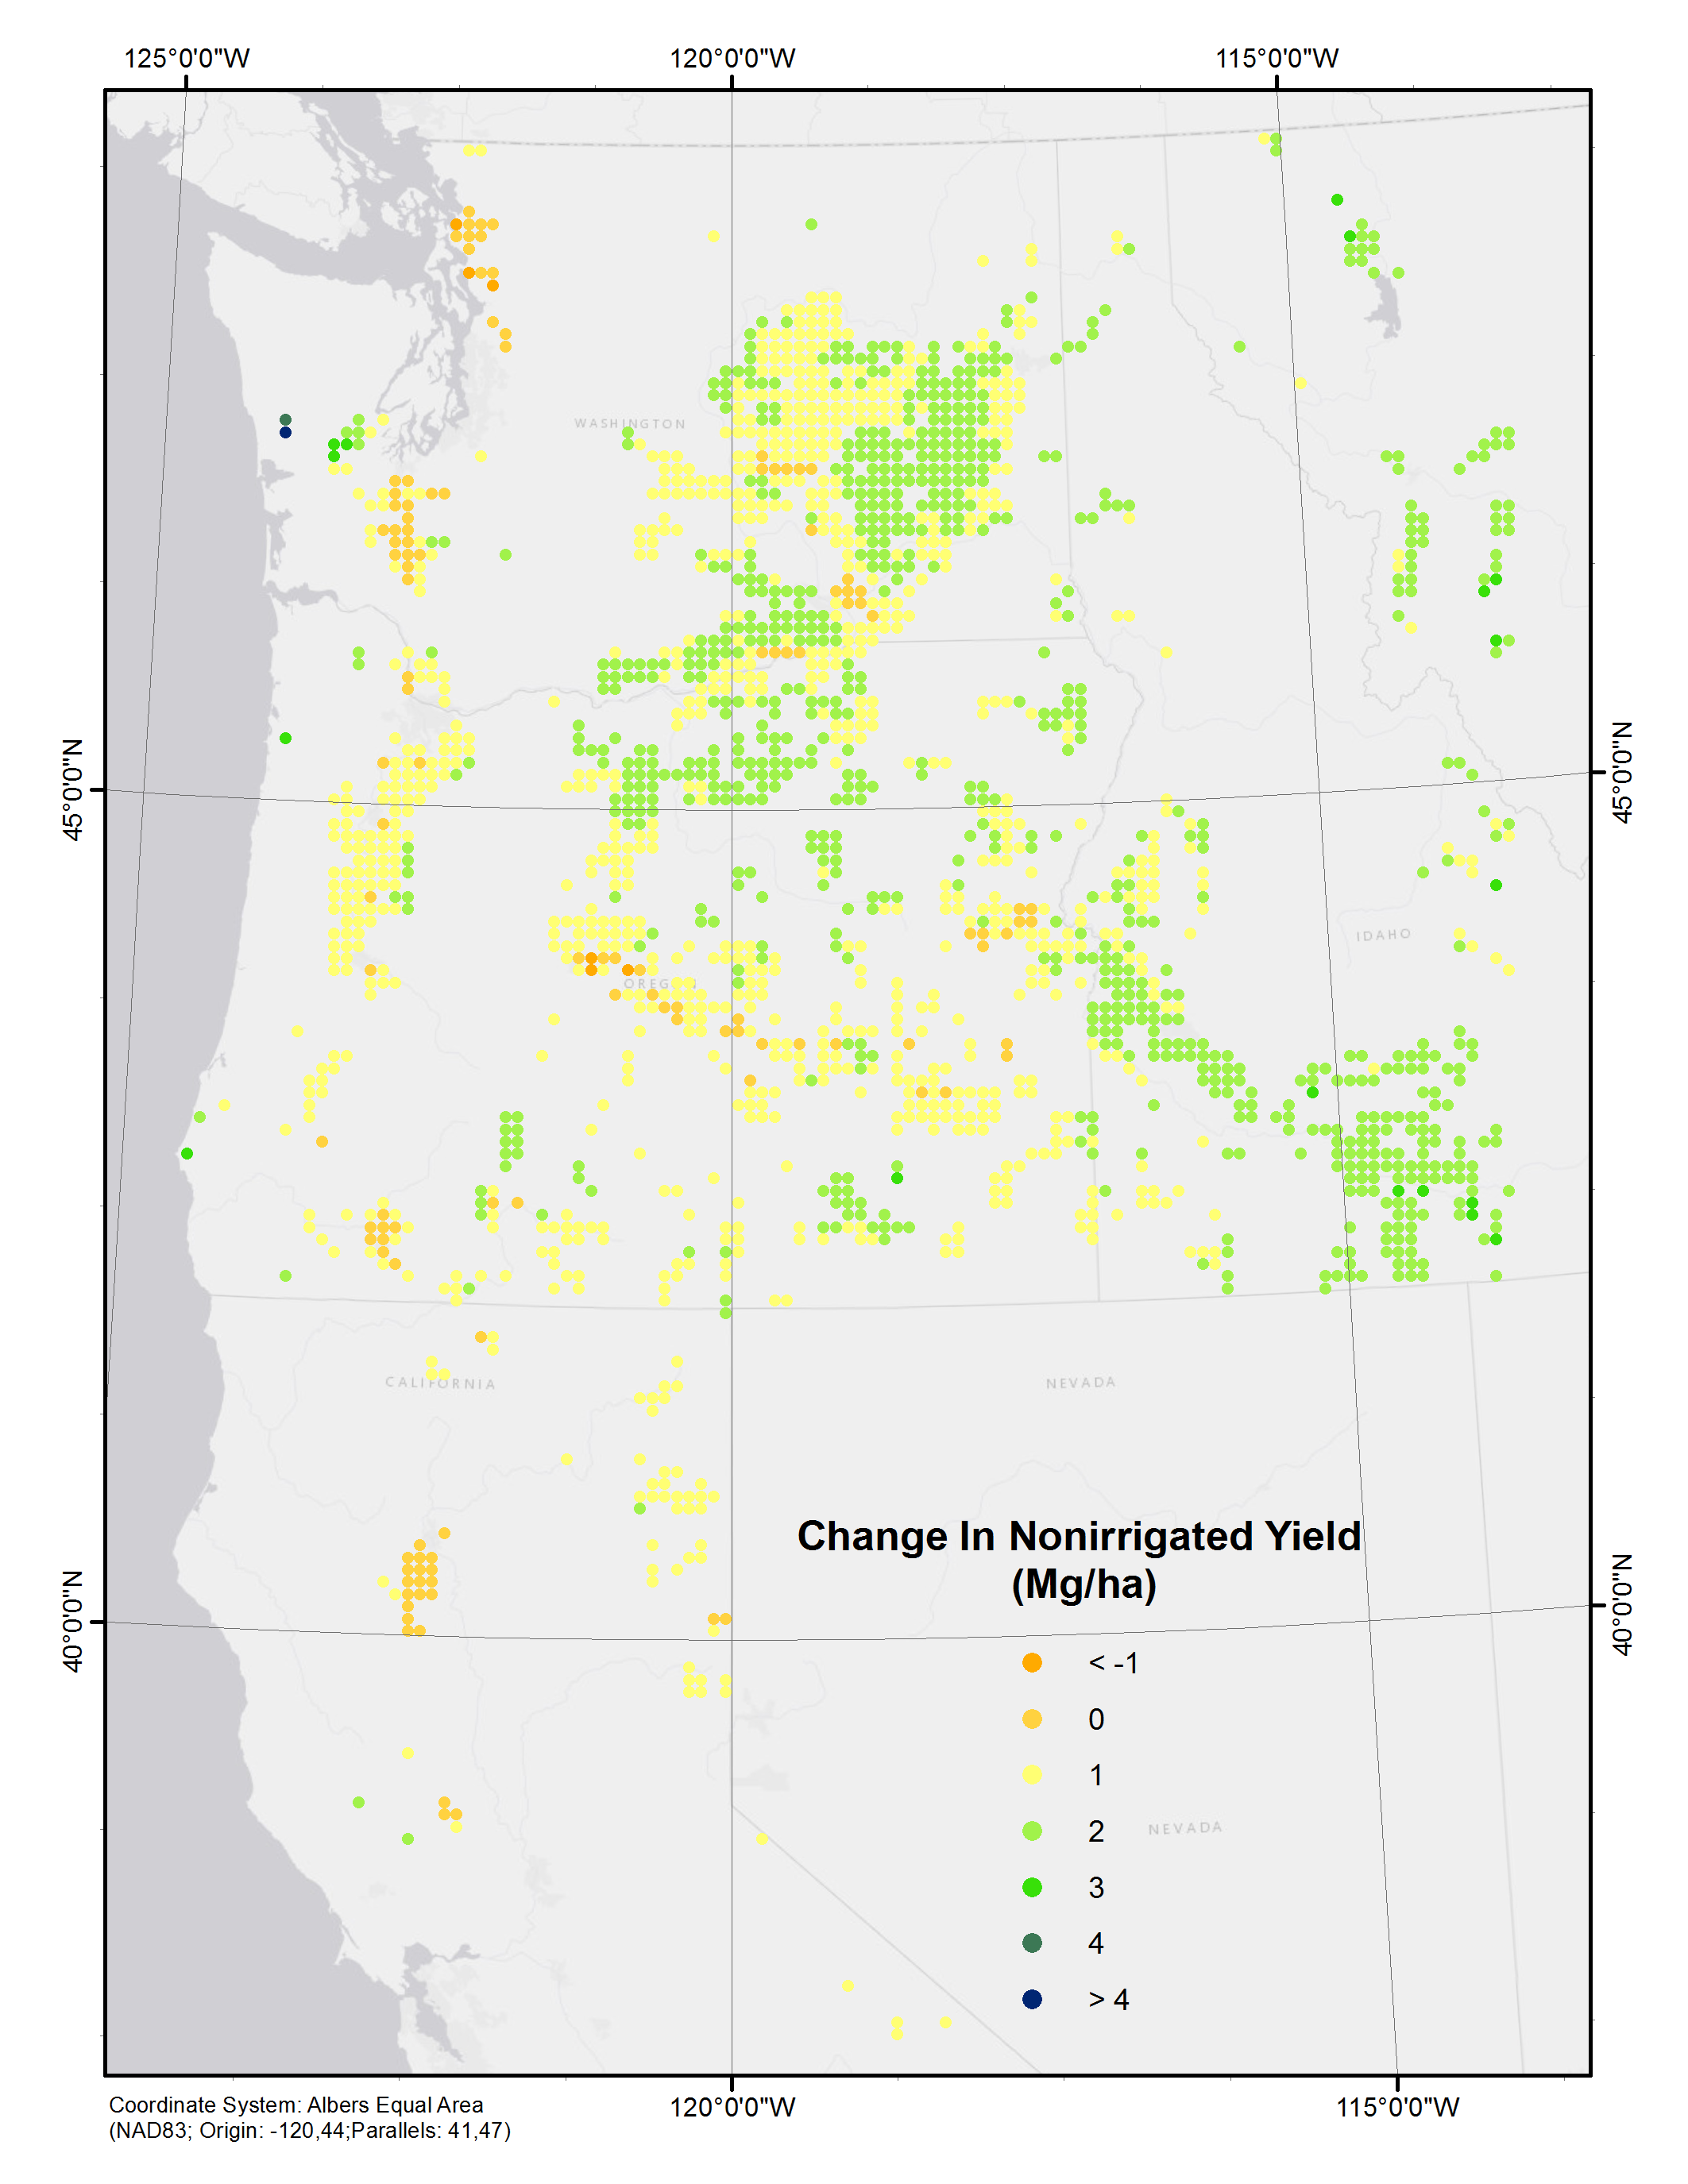
\includegraphics[width=1\linewidth]{climate_nonirrigated}
  \caption{Changes in predicted non-irrigated yield for \ac{IPCC} scenario A1B
    for a plantation planting in 2040-2058.}
  \label{fig:new_nonirrigated}
\end{figure}

These change estimations can inform both the individual farmer in terms of
predicting long term viability of poplar plantations as a \ac{SRWC}
feedstock, as well as regional estimations on the mid-term ability of
such a feedstock to provide an expected harvest, and therefore an
expected level of biofuel production.  Not only changes in expected
overall yields, but changes in the spatial distribution of the yields
can have impacts on economic analysis of a \ac{SRWC} based biofuel
industry in the \ac{PNW}.  

These example climate change yield change predictions are
illustrative, but the mean change in yields are not necessarily the
most robust estimation of changes in yield predictions.  First, the
\ac{CCSM3} models are not tuned to the relatively short time frame of
looking forward 25-50 years.  In addition, while temperature increases
are consistently predicted, the change in precipitation is less
uniformly predicted among different models and scenarios. 

With appropriate input information, the \ac{3pg} model can predict
yields for the entire \ac{PNW} study region, under various irrigation
scenarios.  When linked with models of crop adoption and biorefinery
models the economic viability of poplar as a biofuel feedstock can be
examined.
 
For example, in the \ac{AHB} project, a companion model, the
\acf{BCAM}, predicts price levels where poplar competes with existing
crops in about 35 different general cropping regions in the \ac{PNW}.
The spatially distributed yield predictions inform the \ac{BCAM}
model.  For irrigated land, current yields are input into a \ac{BCAM}
model where they compete with existing crops to determine their
economic viability.  The yield predictions also include predictions in
required water, and the \ac{BCAM} model manages water availability by
balancing any water needs from the poplar with water saved from crops
taken out of the agricultural system.  Outputs of the \ac{BCAM} model
show at what farm gate price (\$/Mg) poplar becomes an economically
viable product.
 
For non-irrigated land, marginal and under utilized lands can be added
into the overall agricultural economy as newly utilized lands.  For
non-irrigated plantations, crop budgets can give estimates of farm gate
costs (\$/Mg) which are affected by the predicted yields.

Both the irrigated and non-irrigated regions, total amount of available
feedstock for a particular farm gate price can then be estimated.
These are also spatially distributed.  Another \ac{AHB} model, the
\acf{GBSM} takes as inputs these spatially distributed price curves,
 and use them in coordination with feedstock transport and refinery
costs, to optimize the size and location of a set of refineries, to
most efficiently process the poplar into a biofuel.  The results from
the \ac{GBSM} model include both the predicted refinery system as well
as an anticipated cost of fuel itself.  The current resolution of the
\ac{AHB} grid is designed to provide a workable input for the solver
of the \ac{GBSM} model.  Subsequent model runs at a finer scale can
test the best scales for application of these models.

\section{Conclusions}
\label{sec:conclude}

With the addition of the coppicing model, the \ac{3pg} model can be
used to predict poplar yields for the \ac{PNW} region.  The model can
include irrigation which increases yields from most areas in the region.  

With additional layers showing current croplands, areas the can be
irrigated are identified.  Poplar suitability maps limit consideration
on non-irrigated plantations to regions that are amenable to such
management.

Limitations of the model presented here are primarily related to
reliability of the predicted yield at the local scale. As the spatial
unit of measure is a 64 km\textsuperscript{2} land area, variability
in growth and yield at a local scale may be great.

Spatially distributed yield predictions inform regional models as to
the expected costs of producing a poplar biofuel feedstock and the
price at which that commodity becomes economically viable.

\section{Acknowledgments}
This work is supported by an Agriculture and Food Research Initiative
Competitive Grant no. 2011-68005-30407 from the USDA National
Institute of Food and Agriculture (NIFA).

%% The Appendices part is started with the command \appendix;
%% appendix sections are then done as normal sections
%% \appendix

%% \section{}
%% \label{}

%% If you have bibdatabase file and want bibtex to generate the
%% bibitems, please use
%%
\bibliographystyle{vancouver} 
\bibliography{ahb-pnw}

%%\input{hart14model-poplar-custom.bbl}

\end{document}
\endinput
%%
%% End of file `elsarticle-template-num.tex'.

%  LocalWords:  dataset Albers landcover postgresql geospatial SQL
%  LocalWords:  postgis PLSQL JavaScript timestep coppicing datasets
%  LocalWords:  biorefinery aboveground coppiced biofuels feedstock
%  LocalWords:  SRWC parameterized physiographic orographic Isolines
%  LocalWords:  isolines parameterizations allometric coppice biofuel
%  LocalWords:  photosynthetically parameterize litterfall insolation
%  LocalWords:  rangeland
